\documentclass[a4paper,12pt]{article} 
% 使用ctex包支持中文
\usepackage[UTF8,heading = true]{ctex}
\usepackage[utf8]{inputenc}
\usepackage[T1]{fontenc}
\usepackage{graphicx}
\usepackage{float}
\usepackage{amsmath}
\usepackage{amsfonts}
\usepackage{amssymb}
\usepackage{booktabs}
\usepackage{multirow}
\usepackage{subcaption}
\usepackage{indentfirst}
\usepackage{geometry}
\usepackage{fancyhdr}
\usepackage{ctex}
\usepackage[labelfont=bf]{caption}
\usepackage{listings}
\usepackage{xcolor} % 用于定义自定义颜色和高亮
\usepackage{ragged2e} % 导入ragged2e宏包,用于支持段落两端对齐
\renewcommand{\figurename}{Figure}

\lstset{
  language=Python,              % 设置语言
  basicstyle=\ttfamily\small,   % 设置基本样式
  keywordstyle=\color{blue},    % 设置关键字样式
  stringstyle=\color{red},      % 设置字符串样式
  commentstyle=\color{green},   % 设置注释样式
  morecomment=[s][\color{magenta}]{from}{import},   % 对特定的关键字进行高亮
  frame=single,                 % 给代码添加框
  rulecolor=\color{black},      % 框的颜色
  numbers=left,                 % 在左侧添加行号
  numberstyle=\tiny\color{gray},% 行号样式
  breaklines=true,              % 自动换行
  postbreak=\mbox{\textcolor{red}{$\hookrightarrow$}\space},
  showstringspaces=false,       % 不特别显示字符串中的空格
  tabsize=2                     % 设置tab为2个空格宽度
}


\geometry{left=3cm,right=3cm,top=3cm,bottom=3cm}

% \ctexset{
%     % 修改 section。
%     section={   
%         name={Experiment,:},
%         number={\arabic{section}},
%         format=\heiti\bfseries\centering\zihao{-2} % 设置 section 标题为黑体、右对齐、小4号字
%     },
%     % 修改 subsection。
%     subsection={   
%         name={,、},
%         number={\arabic{subsection}},
%         format=\bfseries\zihao{4} % 设置 subsection 标题为黑体、5号字
%     },
%     % 修改 subsection。
%     subsubsection={   
%         name={,、},
%         number={\arabic{subsubsection}},
%         format=\bfseries\zihao{-4} % 设置 subsection 标题为黑体、5号字
%     }
% }
\fancyhead{}


\begin{document}

%制作封面
\begin{titlepage}
    \begin{center}
        \par
            \centerline{
\includegraphics[scale=1.5]{data/media/image1.jpeg} 
\includegraphics[scale=3]{data/media/image2.jpeg}} %插入图片
        \par
		\vskip 5cm
		\fontsize{50}{20} 实\quad 验\quad 报\quad 告
		\vskip 10cm

	\begin{tabular}{l}
		\songti \zihao{-2} \bfseries 课程名称:深度学习与计算机视觉
		\quad \\
	    	\songti \zihao{-2} \bfseries 学生姓名:zyh
	    	\quad \\
		\songti \zihao{-2} \bfseries 学生学号:202264691103
		\quad \\
	    	\songti \zihao{-2} \bfseries 学生专业:人工智能
	    	\quad \\
	     \songti \zihao{-2} \bfseries 开课学期:2023-2024年第二学期
	     \quad \\
           \songti \zihao{-2} \bfseries  提交日期:2024年5月10日
    \end{tabular}
    \end{center}
\end{titlepage}


% 生成目录
\newpage
\pagestyle{empty}
\begin{center}
\renewcommand{\contentsname}{Table of Contents}
\tableofcontents
\end{center}

\newpage

\setcounter{page}{1}
Description of the experimental setting:
\begin{lstlisting}
python 3.10.11
torch 2.1.2+cu118
AMD 6900HX + Geforce RTX3070Ti Laptop GPU @8GB
\end{lstlisting}
\textbf{Note: I did not use the \texttt{d2l} library from the textbook, and I only solved the experimental content using the \texttt{torch} library.}

\section{Linear Regression Model}
\subsection{Experimental Purpose}
Designed to define a simple linear regression model so that the model can be read and trained on the data

\subsection{Experimental Principle}
\subsubsection{Linear Regression}
Linear regression output is a continuous value and is therefore suitable for regression problems. Regression problems are common in practice, such as the problem of predicting continuous values of house prices, temperatures, sales, etc. The regression problem is a simple one.
Regression problems are common in practice, such as those that predict continuous values such as house prices, temperatures, sales, etc. Unlike regression problems, the final output of the model in classification problems is a discrete value. Unlike regression problems, the final output of the model in classification problems is a discrete value.
Problems with discrete outputs such as image classification, spam recognition, disease detection, etc. fall into the category of classification problems.
Softmax regression is used for classification problems. Since both linear regression and softmax regression are single-layer neural grids, the concepts and techniques involved are also applicable to most deep learning models.
The concepts and techniques involved in linear regression and softmax regression are also applicable to most deep learning models.

Linear regression is the most basic of the regression models. The predictions of the model can be expressed as follows:

\begin{equation}
\hat{y} = w_1x_1 + \dots + w_dx_d + b
\end{equation}

or expressed in dot product form as:
\begin{equation}
\hat{y} = \mathbf{w}^\top \mathbf{x} + b
\end{equation}
The vector \( \mathbf{x} \) corresponds to the features of a single data sample. The matrix \( \mathbf{X} \in \mathbb{R}^{n \times d} \), represented by symbols, conveniently references the n samples in our entire dataset. Here, each row of \( \mathbf{X} \) represents a sample, and each column represents a feature.

We adopt the squared error function as the loss function. When the prediction for sample \( i \) is \( \hat{y}^{(i)} \) and its corresponding true label is \( y^{(i)} \), the squared error can be defined by the following formula:

\begin{equation}
l^{(i)}(\mathbf{w}, b) = \frac{1}{2} \left( \hat{y}^{(i)} - y^{(i)} \right)^2
\end{equation}

Over the entire dataset, the mean loss can be represented as:

\begin{equation}
L(\mathbf{w}, b) = \frac{1}{n} \sum_{i=1}^{n} l^{(i)}(\mathbf{w}, b) = \frac{1}{n} \sum_{i=1}^{n} \frac{1}{2} \left( \mathbf{w}^\top \mathbf{x}^{(i)} + b - y^{(i)} \right)^2
\end{equation}

During training, the learning objective is to find a set of parameters \( (\mathbf{w}^*, b^*) \) that minimizes the total loss \( L(\mathbf{w}, b) \):

\begin{equation}
\mathbf{w}^*, b^* = \underset{\mathbf{w}, b}{\mathrm{argmin}} \ L(\mathbf{w}, b)
\end{equation}

\subsection{Experimental Content}
\subsubsection{Generate and Read Data Sets}
This part includes generating synthetic data and loading the dataset.
\begin{lstlisting}
import torch
from torch import nn
import torch.optim as optim
import numpy as np

# Helper functions
def synthetic_data(w, b, num_examples):
    features = torch.normal(0, 1, (num_examples, len(w)))
    labels = torch.matmul(features, w) + b
    labels += torch.normal(0, 0.01, labels.shape)
    return features, labels

def load_array(data_arrays, batch_size, shuffle=True):
    dataset = torch.utils.data.TensorDataset(*data_arrays)
    return torch.utils.data.DataLoader(dataset, batch_size=batch_size, shuffle=shuffle)

true_w = torch.tensor([2, -3.4], dtype=torch.float32)
true_b = 4.2
features, labels = synthetic_data(true_w, true_b, 1000)

batch_size = 10
data_iter = load_array((features, labels), batch_size)
\end{lstlisting}

\subsubsection{Define the model and initialize the parameters}
This part includes defining the linear regression model and initializing the model parameters.
\begin{lstlisting}
# Define the linear regression model
net = nn.Sequential(nn.Linear(2, 1))  # 2 inputs (features) and 1 output (prediction)

# Initialize model parameters
nn.init.normal_(net[0].weight, std=0.01)
nn.init.constant_(net[0].bias, val=0)
\end{lstlisting}

\subsubsection{Training Model}
This part includes setting up the loss function, optimizer, and performing model training.
\begin{lstlisting}
# Loss function
loss = nn.MSELoss()

# Optimizer
trainer = optim.SGD(net.parameters(), lr=0.02)

num_epochs = 3
for epoch in range(num_epochs):
    for X, y in data_iter:
        # Forward pass
        output = net(X)
        l = loss(output, y.view(-1, 1))  # Compute loss

        # Backward pass
        trainer.zero_grad()
        l.backward()
        trainer.step()

    # Calculate the loss on the entire dataset
    l = loss(net(features), labels.view(-1, 1))
    print(f'epoch {epoch + 1}, loss: {l.item()}')
\end{lstlisting}

\subsubsection{Result Output}
This part consists of comparing the estimated model parameters with the true parameters and outputting the results.
\begin{lstlisting}
# Compare estimated parameters with true parameters
w = net[0].weight.data.numpy()
print('Error in estimating w', true_w.numpy() - w.flatten())
b = net[0].bias.data.numpy()
print('Error in estimating b', true_b - b.item())
\end{lstlisting}

\subsection{Results}
After 10 epochs of training on this simple data and model.
\begin{lstlisting}
epoch 1, loss: 0.01113776583224535
epoch 2, loss: 0.00010264442971674725
epoch 3, loss: 9.953241533366963e-05
epoch 4, loss: 9.929583757184446e-05
epoch 5, loss: 9.907934145303443e-05
epoch 6, loss: 9.957896691048518e-05
epoch 7, loss: 9.958783630281687e-05
epoch 8, loss: 9.92832938209176e-05
epoch 9, loss: 9.910028165904805e-05
epoch 10, loss: 9.921971650328487e-05
\end{lstlisting}

for the computational error of w vs. b:
\begin{lstlisting}
Error in estimating w [0.00047803 0.00022626]
Error in estimating b 0.0006668090820314276
\end{lstlisting}
\subsection{Experiment Summary}
Based on the training results, the following experimental conclusions can be drawn:

\subsubsection{Convergence Analysis (math.)}
\begin{itemize}
  \item The loss (loss) of the model on the training data decreases as the training period increases (epoch increases).
  \item The initial loss is high, and as training proceeds, the loss decreases rapidly, reaching a very low level after the first epoch.
  \item In the subsequent epochs, the loss basically stays at a stable level with little change, indicating that the model is close to convergence.
\end{itemize}

\subsubsection{Model Performance Analysis}
\begin{itemize}
\item The final post-training loss is very small, around 0.0001 or so, indicating that the model achieved a good fit on the training data.
\item The lower loss means that the model is able to accurately predict the labeled values in the synthetic data.
\end{itemize}

\subsubsection{Model Parameter Estimation}
\begin{itemize}
  \item The accuracy of the model can be assessed by comparing the errors of the estimated model parameters (weights \( w \) and biases \( b \)) with the true parameters.
  \item Usually, the better the model is trained, the smaller the error between the estimated and true parameters.
\end{itemize}

\subsubsection{Experiment Summary}


\begin{itemize}
  \item With this experiment, we successfully trained a simple linear regression model to make accurate predictions on synthetic data.
  \item The training loss of the model is low, indicating that the model has good generalization ability and can be used for prediction on unknown data.
\end{itemize}
   
\newpage
\section{Softmax Regression Model}
\subsection{Experimental Purpose}
Designing softmax regression models to implement a multi-category classification task on the Fashion-MNIST dataset.
\subsection{Experimental Principle}
\subsubsection{Softmax Network Structure}
In a classification problem, you need to use a model with multiple outputs, each corresponding to an affine function. If the number of features is 4 and there are 3 classification categories, you would compute three *unnormalized predictions* (logits) for each input: \( o_1 \), \( o_2 \), and \( o_3 \).

\begin{equation}
\begin{split}
o_1 &= x_1w_{11} + x_2w_{12} + x_3w_{13} + x_4w_{14} + b_1, \\
o_2 &= x_1w_{21} + x_2w_{22} + x_3w_{23} + x_4w_{24} + b_2, \\
o_3 &= x_1w_{31} + x_2w_{32} + x_3w_{33} + x_4w_{34} + b_3.
\end{split}
\end{equation}
The three outputs \( o_1 \), \( o_2 \), and \( o_3 \) represent the output layer of softmax regression. They serve as a fully connected layer representing the raw prediction values for each class before normalization.

\subsubsection{Softmax Operation}
For classification purposes, the output of the model $\hat{y}_j$ can be thought of as the probability of belonging to class $j$, with all outputs being
non-negative and summing to 1. The softmax function is used to achieve exactly this one goal.

\begin{equation}
\hat{y} = \text{softmax}(\mathbf{o}) \quad \text{included among these} \quad \hat{y}_j = \frac{\exp(o_j)}{\sum_k \exp(o_k)}
\end{equation}

Here, for all j there is always $0 \leq \hat{y}_j \leq 1$. Thus, $\hat{\mathbf{y}}$ can be considered a correct probability distribution.
The softmax operation does not change the order of magnitude between the unnormalized predictions $\mathbf{o}$, it only determines the order of magnitude assigned to each of the class
probability to each category. Thus the optimization objective remains during the prediction process:

\begin{equation}
\underset{j}{\mathrm{argmax}} \ \hat{y}_j = \underset{j}{\mathrm{argmax}} \ o_j
\end{equation}

\subsubsection{Loss Function}
The softmax function implements a simple \(\hat{\mathbf{y}}\) as the conditional probability of the class given the input \(\mathbf{x}\).For example, \(\hat{y_1} = P(y = \text{cat} \, | \, \mathbf{x})\). Assume that the entire dataset is \(\{\mathbf{X}, \mathbf{Y}\}\) and there are \(n\) samples, where samples indexed \(i\) consist of a feature vector \(\mathbf{x}^{(i)}\) and a vector of unique heat labels \(\mathbf{y}^{(i)}\). The calculated probability values are compared:

\begin{equation}
P(Y | X) = \prod_{i=1}^{n} P(y^{(i)} | x^{(i)})
\end{equation}

Maximizing $P(\mathbf{Y} \,| \, \mathbf{X})$ according to maximum likelihood estimation is equivalent to minimizing the negative log-likelihood:
\begin{equation}
-\log P(Y | X) = \sum_{i=1}^{n} -\log P(y^{(i)} | x^{(i)}) = \sum_{i=1}^{n} l(y^{(i)}, \hat{y}^{(i)})
\end{equation}

where the loss function is, for any label $\mathbf{y}$ and model prediction $\hat{\mathbf{y}}$:
\begin{equation}
l(y, \hat{y}) = - \sum_{j=1}^{q} y_j \log \hat{y}_j
\end{equation}
Since $\mathbf{y}$ is a uniquely thermally encoded vector of length q, all terms j vanish except for one term
up. Since all $\hat{y}_j$ are predicted probabilities, their logarithms are never greater than 0. Thus, if the
correctly predicts the actual label, i.e., if the actual label $P(\mathbf{y} \,| \, \mathbf{x}) = 1$, then the loss function cannot be further minimized
minimization. Note that this is often not possible. For example, there may be labeling noise in the dataset (e.g., some samples
may be mislabeled), or the input features do not have enough information to perfectly classify each sample.

\subsection{Experimental Content}
\subsubsection{Data loading and Pre-processing}
This part includes loading the Fashion MNIST dataset and pre-processing it.
\begin{lstlisting}
import torch
from torchvision import datasets, transforms

def load_data_fashion_mnist(batch_size, resize=None):
    # 定义数据预处理操作
    trans = [transforms.ToTensor()]
    if resize:
        trans.insert(0, transforms.Resize(resize))
    trans = transforms.Compose(trans)

    # 加载训练集和测试集
    mnist_train = datasets.FashionMNIST(root="./data", train=True, transform=trans, download=True)
    mnist_test = datasets.FashionMNIST(root="./data", train=False, transform=trans, download=True)

    # 创建 DataLoader
    train_loader = torch.utils.data.DataLoader(mnist_train, batch_size=batch_size, shuffle=True)
    test_loader = torch.utils.data.DataLoader(mnist_test, batch_size=batch_size, shuffle=False)

    return train_loader, test_loader
\end{lstlisting}

\subsubsection{Define the Neural Network Model}
This section includes defining the neural network model used for Fashion MNIST classification.
\begin{lstlisting}
import torch
from torch import nn

class FashionMNISTModel(nn.Module):
    def __init__(self):
        super(FashionMNISTModel, self).__init__()
        self.flatten = nn.Flatten()
        self.linear = nn.Linear(28*28, 10)

    def forward(self, x):
        x = self.flatten(x)
        x = self.linear(x)
        return x

\end{lstlisting}

\subsubsection{Model Training and Evaluation}
This part includes the training and evaluation functions of the model.
\begin{lstlisting}
import torch

# Train the model with loss curve, train accuracy, and test accuracy visualization
def train(model, train_loader, criterion, optimizer, num_epochs):
    model.train()
    train_losses = []
    train_accuracies = []
    for epoch in range(num_epochs):
        running_loss = 0.0
        correct = 0
        total = 0
        for images, labels in train_loader:
            images, labels = images.to(device), labels.to(device)
            optimizer.zero_grad()
            outputs = model(images)
            loss = criterion(outputs, labels)
            loss.backward()
            optimizer.step()
            running_loss += loss.item() * images.size(0)
            
            _, predicted = torch.max(outputs.data, 1)
            total += labels.size(0)
            correct += (predicted == labels).sum().item()

        epoch_loss = running_loss / len(train_loader.dataset)
        train_losses.append(epoch_loss)
        train_accuracy = correct / total
        train_accuracies.append(train_accuracy)
        
        print(f"Epoch {epoch + 1}, Loss: {epoch_loss:.4f}, Train Accuracy: {train_accuracy:.4f}")

    # Plot the training loss curve and train accuracy curve
    plt.figure(figsize=(10, 4))
    plt.subplot(1, 2, 1)
    plt.plot(range(1, num_epochs + 1), train_losses, label='Training Loss')
    plt.title('Training Loss over Epochs')
    plt.xlabel('Epoch')
    plt.ylabel('Loss')
    plt.legend()

    plt.subplot(1, 2, 2)
    plt.plot(range(1, num_epochs + 1), train_accuracies, label='Training Accuracy', color='orange')
    plt.title('Training Accuracy over Epochs')
    plt.xlabel('Epoch')
    plt.ylabel('Accuracy')
    plt.legend()
    plt.show()


def evaluate(model, test_loader):
    model.eval()
    correct = 0
    total = 0
    with torch.no_grad():
        for images, labels in test_loader:
            images, labels = images.to(device), labels.to(device)
            outputs = model(images)
            _, predicted = torch.max(outputs.data, 1)
            total += labels.size(0)
            correct += (predicted == labels).sum().item()
    accuracy = correct / total
    print(f"Test Accuracy: {accuracy:.3f}")
\end{lstlisting}

\subsubsection{Model Prediction and Visualization}
This part consists of making predictions using the trained model and visualizing some of the predictions.
\begin{lstlisting}
import matplotlib.pyplot as plt

def predict(model, test_loader):
    model.eval()
    with torch.no_grad():
        for images, labels in test_loader:
            images, labels = images.to(device), labels.to(device)
            outputs = model(images)
            _, predicted = torch.max(outputs.data, 1)
            break

    # 显示部分预测结果
    fig, axes = plt.subplots(3, 3, figsize=(8, 8))
    for i, ax in enumerate(axes.flat):
        ax.imshow(images[i].cpu().numpy().squeeze(), cmap="gray")
        ax.set_title(f"True: {labels[i].item()}\nPredicted: {predicted[i].item()}")
        ax.axis("off")
    plt.show()
\end{lstlisting}

\subsubsection{Main Program Running}
\begin{lstlisting}
import torch
from torchvision import datasets, transforms

# 加载数据
batch_size = 256
train_loader, test_loader = load_data_fashion_mnist(batch_size)

# 定义模型并移动到GPU
device = torch.device("cuda" if torch.cuda.is_available() else "cpu")
model = FashionMNISTModel().to(device)

# 定义损失函数和优化器
criterion = nn.CrossEntropyLoss()
optimizer = torch.optim.SGD(model.parameters(), lr=0.1)

# 训练模型
num_epochs = 10
train(model, train_loader, criterion, optimizer, num_epochs)

# 评估模型
evaluate(model, test_loader)

# 进行预测并可视化结果
predict(model, test_loader)
\end{lstlisting}

\subsection{Results}
In this experiment, 10 epochs were trained at a learning rate of 0.1.The results are as follows.
\begin{lstlisting}
Epoch 1, Loss: 0.7814, Train Accuracy: 0.7559
Epoch 2, Loss: 0.5706, Train Accuracy: 0.8135
Epoch 3, Loss: 0.5269, Train Accuracy: 0.8247
Epoch 4, Loss: 0.5020, Train Accuracy: 0.8315
Epoch 5, Loss: 0.4856, Train Accuracy: 0.8368
Epoch 6, Loss: 0.4743, Train Accuracy: 0.8397
Epoch 7, Loss: 0.4658, Train Accuracy: 0.8425
Epoch 8, Loss: 0.4592, Train Accuracy: 0.8438
Epoch 9, Loss: 0.4522, Train Accuracy: 0.8463
Epoch 10, Loss: 0.4471, Train Accuracy: 0.8476
\end{lstlisting}

The loss of training versus the change in accuracy is shown below:

% 去掉figure环境,直接插入图像
\centering % 如果需要居中对齐图像
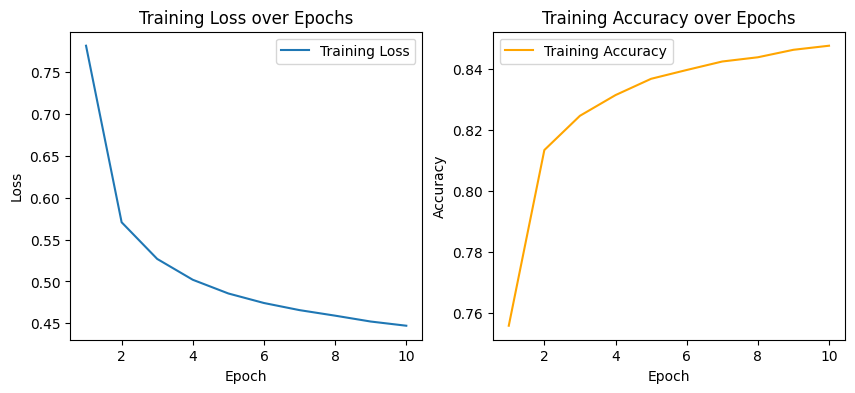
\includegraphics[width=0.8\linewidth]{images/lab1_2_loss.png}
\captionof{figure}{Training Accuracy and Loss Value} % 使用\captionof命令添加标题


% 插入另一张图
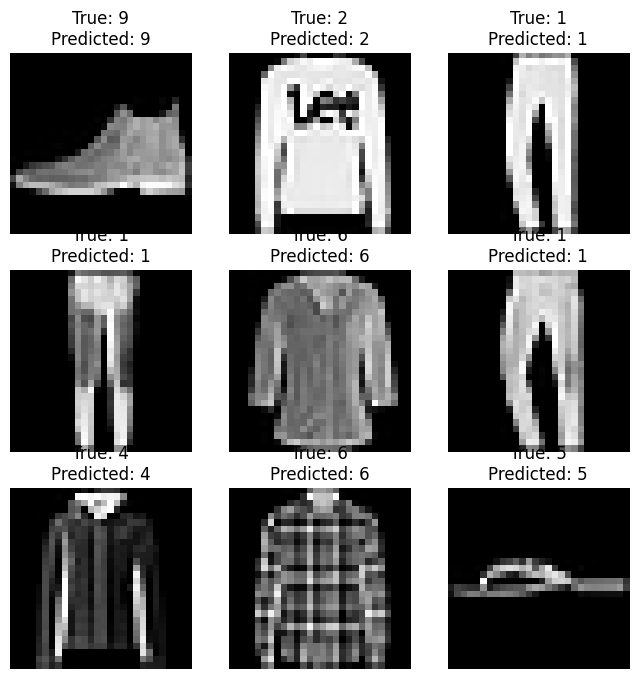
\includegraphics[width=0.8\linewidth]{images/lab1_2_result.png}
\captionof{figure}{Model prediction results}

\justifying
\subsection{Experiment Summary}
\subsubsection{Analysis of the training process}
Training Loss:
As the training epoch increases, the loss of the model on the training set gradually decreases, from 0.7814 at the beginning to 0.4471 at the end.
The continuous decrease of the loss indicates that the model is gradually optimized during the learning process, and the fitting effect on the training data is gradually improved.
Training Accuracy:
The training accuracy gradually increases with the increase of training epoch, from about 75.59\% at the beginning to about 84.76\% at the end.
The increase in accuracy indicates that the model gradually learns the features and patterns of the data during the training process, and is able to classify and predict the training samples more accurately.

\subsubsection{Model Performance Evaluation}
Test Accuracy:
The trained model achieved an accuracy of about 84.76\% on the test set.
The test accuracy is similar to the training accuracy, indicating that the model has good generalization ability and can effectively predict unseen test samples.

\subsubsection{Results}
In this experiment, we trained a simple neural network model that achieved good training and testing performance on the Fashion MNIST dataset.
As the training progresses, the loss of the model gradually decreases, while the training and testing accuracy gradually increases, indicating that the model effectively improves its ability to recognize clothing images during the learning process.
The final test accuracy is about 84.76\%, which indicates that the model is able to recognize the clothing categories in the Fashion MNIST dataset successfully to some extent.

\newpage
\section{Multi-layer Perceptron}
\subsection{Experimental Purpose}
Design of a multilayer perceptron model to implement a multi-category classification task on the Fashion-MNIST dataset.
\subsection{Experimental Principle}
\subsubsection{Model Hidden Layer}
We can overcome the limitations of linear models by adding one or more hidden layers to the network, making it
can handle more general types of functional relationships. The easiest way to do this is to stack many fully connected layers
on top of each other. Each layer outputs to the layer above it until the final output is generated. We can think of the first L-1 layers
as a representation and the last layer as a linear predictor. This architecture is often referred to as a multilayer perceptron.
perceptron.)

A small batch of n samples is represented by the matrix $\mathbf{X} \in \mathbb{R}^{n \times d}$, where each sample has d input
Features. For a single hidden layer multilayer perceptual machine with $h$ hidden units, the output of the hidden layer is denoted by $\mathbf{H} \in \mathbb{R}^{n \times d}$, which is called the hidden representation.
The outputs are called hidden representations. In math or code, $\mathbf{H}$ is also called a hidden-layer variable.
hidden-layer variable or hidden variable. Because both the hidden layer and the output
layers are fully connected, we have hidden-layer weights $\mathbf{W}^{(1)} \in \mathbb{R}^{d \times h}$ and hidden-layer biases $\mathbf{b}^{(1)} \in \mathbb{R}^{1 \times h}$
and the output layer weights $\mathbf{W}^{(2)} \in \mathbb{R}^{h \times q}$ and the output layer bias $\mathbf{b}^{(2)} \in \mathbb{R}^{1 \times q}$. Formally, we proceed as follows
Formally, we compute the output of the single hidden layer multilayer perceptron $\mathbf{O}^{(2)} \in \mathbb{R}^{n \times q}$:

\begin{equation}
\begin{split}
\mathbf{H} = \mathbf{XW}^{(1)} + \mathbf{b}^{(1)},\\
\mathbf{O} = \mathbf{HW}^{(2)} + \mathbf{b}^{(2)}.
\end{split}
\end{equation}

\subsubsection{Activation Function}
The activation function $\sigma$ enhances the nonlinear performance of the model and prevents the multilayer perceptron model from degenerating into a linear model.

\begin{equation}
\begin{split}
\mathbf{H} = \sigma(\mathbf{XW}^{(1)} + \mathbf{b}^{(1)}), \\
\mathbf{O} = \mathbf{HW}^{(2)} + \mathbf{b}^{(2)}.
\end{split}
\end{equation}

In machine learning, there are several common activation functions:

1. ReLU Function

Given an element \( x \), the ReLU function is defined as the maximum of that element and 0:
\begin{equation}
\text{ReLu}(x) = \text{max}(x,0)
\end{equation}
The ReLU function sets the corresponding activation value to 0, keeping only positive elements and discarding all negative elements.

2. Sigmoid Function

The sigmoid function transforms its input to an output in the range (0, 1). It compresses any input from the range (-inf, inf) to some value within the range (0, 1):
\begin{equation}
\text{sigmoid}(x) = \frac{1}{1 + \exp(-x)}.
\end{equation}

3. Tanh Function

Similar to the sigmoid function, the tanh (hyperbolic tangent) function also compresses its input to the range (-1, 1). The formula for the tanh function is:
\begin{equation}
\tanh(x) = \frac{1 - \exp(-2x)}{1 + \exp(-2x)}.
\end{equation}
Compared to the sigmoid function, it is neutral symmetric about the origin of the coordinate system, making it better suited for handling negative data values.

\subsection{Experimental Content}
\subsubsection{Data loading and Pre-processing}
The first section is responsible for loading and preprocessing the Fashion MNIST dataset.Fashion MNIST is a dataset commonly used for image categorization and contains grayscale images of different categories, such as clothes and shoes. When loading the data, we use \texttt{torchvision.datasets.FashionMNIST} to obtain the training and test sets. If the dataset has not been downloaded to the specified path (\texttt{root='. /data'}), it will be downloaded automatically.

Next, we created a transformation pipeline (\texttt{transforms}) using \texttt{transforms.Compose}, which consists of two main preprocessing steps:

\begin{itemize}
    \item \texttt{transforms.ToTensor()}: converts the image to PyTorch's tensor format. This step converts a PIL image or numpy array into a tensor for subsequent neural network model processing.
    
    \item \texttt{transforms.Normalize((0.5,), (0.5,))}: normalizes the image. This step scales the image pixel values to the range of [-1, 1] by subtracting the mean (0.5) and dividing by the standard deviation (0.5), which helps to improve the stability of the model training and convergence speed.
\end{itemize}

Finally, the preprocessed training and test sets are encapsulated into iterable data loaders using \texttt{torch.utils.data.DataLoader} for subsequent model training and testing. The steps of data loading and preprocessing are critical to the training of deep learning models, and effective data processing can improve the performance and generalization of the model to ensure that the model can effectively learn and generalize to new data samples.

\begin{lstlisting}
import torch
import torchvision
import torchvision.transforms as transforms

def load_data_fashion_mnist(batch_size):
    # 定义数据预处理的转换
    transform = transforms.Compose([
        transforms.ToTensor(),  # 转换为张量
        transforms.Normalize((0.5,), (0.5,))  # 标准化处理
    ])

    # 加载 Fashion MNIST 数据集
    train_dataset = torchvision.datasets.FashionMNIST(root='./data', train=True, download=True, transform=transform)
    test_dataset = torchvision.datasets.FashionMNIST(root='./data', train=False, download=True, transform=transform)

    # 创建数据加载器
    train_loader = torch.utils.data.DataLoader(train_dataset, batch_size=batch_size, shuffle=True)
    test_loader = torch.utils.data.DataLoader(test_dataset, batch_size=batch_size, shuffle=False)

    return train_loader, test_loader

\end{lstlisting}

\subsubsection{Define Neural Network Model}

The second section defines a simple neural network model \texttt{FashionMNISTModel} for the image classification task in the Fashion MNIST dataset. This model contains two linear layers (\texttt{nn.Linear}), which are fully connected layers from the input layer to the hidden layer (\texttt{self.fc1}) and from the hidden layer to the output layer (\texttt{self.fc2}). In the initialization method of the model (\texttt{\_\_init\_\_}), we specify the number of input features (28*28, i.e., the size of the image) and the number of output features (256) for the hidden layer, as well as the number of categories for the output layer (10, which corresponds to the number of categories in the Fashion MNIST dataset). In the forward propagation method (\texttt{forward}), the image is first flattened into a one-dimensional vector, and then processed through the hidden and output layers to produce the final output category score.

This simple neural network model is a standard fully-connected neural network with linear transformation and activation function (\texttt{ReLU}) for image feature extraction and classification. The structure of the model is simple and straightforward and is suitable for image classification tasks dealing with the Fashion MNIST dataset.

\begin{lstlisting}
import torch.nn as nn

class FashionMNISTModel(nn.Module):
    def __init__(self):
        super(FashionMNISTModel, self).__init__()
        self.fc1 = nn.Linear(28*28, 256)  # 第一个全连接层
        self.fc2 = nn.Linear(256, 10)     # 第二个全连接层

    def forward(self, x):
        x = x.view(x.size(0), -1)        # 展平输入图像
        x = torch.relu(self.fc1(x))       # 第一个全连接层使用ReLU激活函数
        x = self.fc2(x)                   # 第二个全连接层输出类别分数
        return x

\end{lstlisting}

\subsubsection{Load Data}

\begin{lstlisting}
import torch.optim as optim

batch_size = 256
train_loader, test_loader = load_data_fashion_mnist(batch_size)

device = torch.device("cuda" if torch.cuda.is_available() else "cpu")
model = FashionMNISTModel().to(device)

criterion = nn.CrossEntropyLoss()
optimizer = optim.SGD(model.parameters(), lr=0.5)

\end{lstlisting}

\subsubsection{Define Training Functions and Test Functions}
The fourth section defines the functions for model training and testing. First is the training function, which receives the model, training data loader, loss function, optimizer and number of training rounds as input parameters. In the training function, the model is set to training mode (\texttt{model.train()}) and then iterated for each training batch. For each batch, the data is first moved to the device (GPU or CPU) and then passed through the model for forward propagation, computation of loss, backpropagation, and optimization of parameters. At the end of each epoch, the average loss value is calculated and output.

Next is the test function (\texttt{test}), which is used to evaluate the performance of the model on a test set. In the test function, the model is set to evaluation mode (\texttt{model.eval()}), disabling gradient computation. Each test batch is then iterated, samples on the test set are predicted and accuracy is calculated. The final output is the accuracy of the model on the test set.

\begin{lstlisting}
def train(model, train_loader, criterion, optimizer, num_epochs):
    model.train()
    for epoch in range(num_epochs):
        running_loss = 0.0
        for images, labels in train_loader:
            images, labels = images.to(device), labels.to(device)
            optimizer.zero_grad()
            outputs = model(images)
            loss = criterion(outputs, labels)
            loss.backward()
            optimizer.step()
            running_loss += loss.item() * images.size(0)
        epoch_loss = running_loss / len(train_loader.dataset)
        print(f"Epoch {epoch + 1}, Loss: {epoch_loss:.4f}")

def test(model, test_loader):
    model.eval()
    correct = 0
    total = 0
    with torch.no_grad():
        for images, labels in test_loader:
            images, labels = images.to(device), labels.to(device)
            outputs = model(images)
            _, predicted = torch.max(outputs.data, 1)
            total += labels.size(0)
            correct += (predicted == labels).sum().item()
    accuracy = correct / total
    print(f"Test Accuracy: {accuracy:.3f}")
\end{lstlisting}

\subsubsection{Training Model}
\begin{lstlisting}
num_epochs = 25
train(model, train_loader, criterion, optimizer, num_epochs)
test(model, test_loader)
\end{lstlisting}

\subsubsection{Visualization of Predicted Results}
\begin{lstlisting}
import matplotlib.pyplot as plt

def visualize_predictions(model, test_loader, device, num_images=10):
    model.eval()
    with torch.no_grad():
        fig, axes = plt.subplots(1, num_images, figsize=(20, 2))

        for i, (images, labels) in enumerate(test_loader):
            images, labels = images.to(device), labels.to(device)
            outputs = model(images)
            _, predicted = torch.max(outputs, 1)

            for j in range(num_images):
                ax = axes[j]
                ax.imshow(images[j].cpu().numpy().squeeze(), cmap='gray')
                ax.set_title(f"True: {labels[j].item()}\nPredicted: {predicted[j].item()}")
                ax.axis('off')

            break  # 只显示第一个批次的部分图像

        plt.show()

# 使用训练好的模型进行可视化预测
visualize_predictions(model, test_loader, device)
\end{lstlisting}

\subsection{Results}
In this experiment, 25 epochs were trained with a learning rate of 0.1.The results are as follows.
\begin{lstlisting}
Epoch 1, Train Loss: 0.6694, Test Accuracy: 0.802
Epoch 2, Train Loss: 0.4653, Test Accuracy: 0.825
Epoch 3, Train Loss: 0.4234, Test Accuracy: 0.823
Epoch 4, Train Loss: 0.3956, Test Accuracy: 0.838
Epoch 5, Train Loss: 0.3751, Test Accuracy: 0.846
Epoch 6, Train Loss: 0.3544, Test Accuracy: 0.843
Epoch 7, Train Loss: 0.3427, Test Accuracy: 0.860
Epoch 8, Train Loss: 0.3319, Test Accuracy: 0.850
Epoch 9, Train Loss: 0.3241, Test Accuracy: 0.864
Epoch 10, Train Loss: 0.3153, Test Accuracy: 0.865
Epoch 11, Train Loss: 0.3031, Test Accuracy: 0.850
Epoch 12, Train Loss: 0.2991, Test Accuracy: 0.858
Epoch 13, Train Loss: 0.2897, Test Accuracy: 0.859
Epoch 14, Train Loss: 0.2832, Test Accuracy: 0.855
Epoch 15, Train Loss: 0.2767, Test Accuracy: 0.874
Epoch 16, Train Loss: 0.2730, Test Accuracy: 0.855
Epoch 17, Train Loss: 0.2666, Test Accuracy: 0.881
Epoch 18, Train Loss: 0.2620, Test Accuracy: 0.855
Epoch 19, Train Loss: 0.2561, Test Accuracy: 0.865
Epoch 20, Train Loss: 0.2524, Test Accuracy: 0.875
Epoch 21, Train Loss: 0.2466, Test Accuracy: 0.872
Epoch 22, Train Loss: 0.2427, Test Accuracy: 0.857
Epoch 23, Train Loss: 0.2380, Test Accuracy: 0.879
Epoch 24, Train Loss: 0.2340, Test Accuracy: 0.860
Epoch 25, Train Loss: 0.2322, Test Accuracy: 0.868
\end{lstlisting}

The loss of training versus the change in accuracy is shown below:

% 去掉figure环境,直接插入图像
\centering % 如果需要居中对齐图像
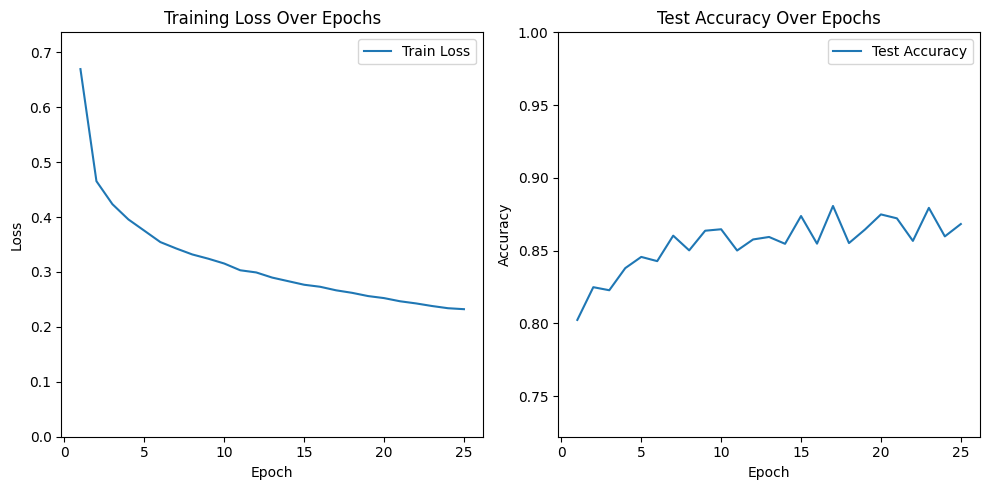
\includegraphics[width=0.8\linewidth]{images/lab1_3_loss.png}
\captionof{figure}{Training Accuracy and Loss Value} % 使用\captionof命令添加标题


% 插入另一张图
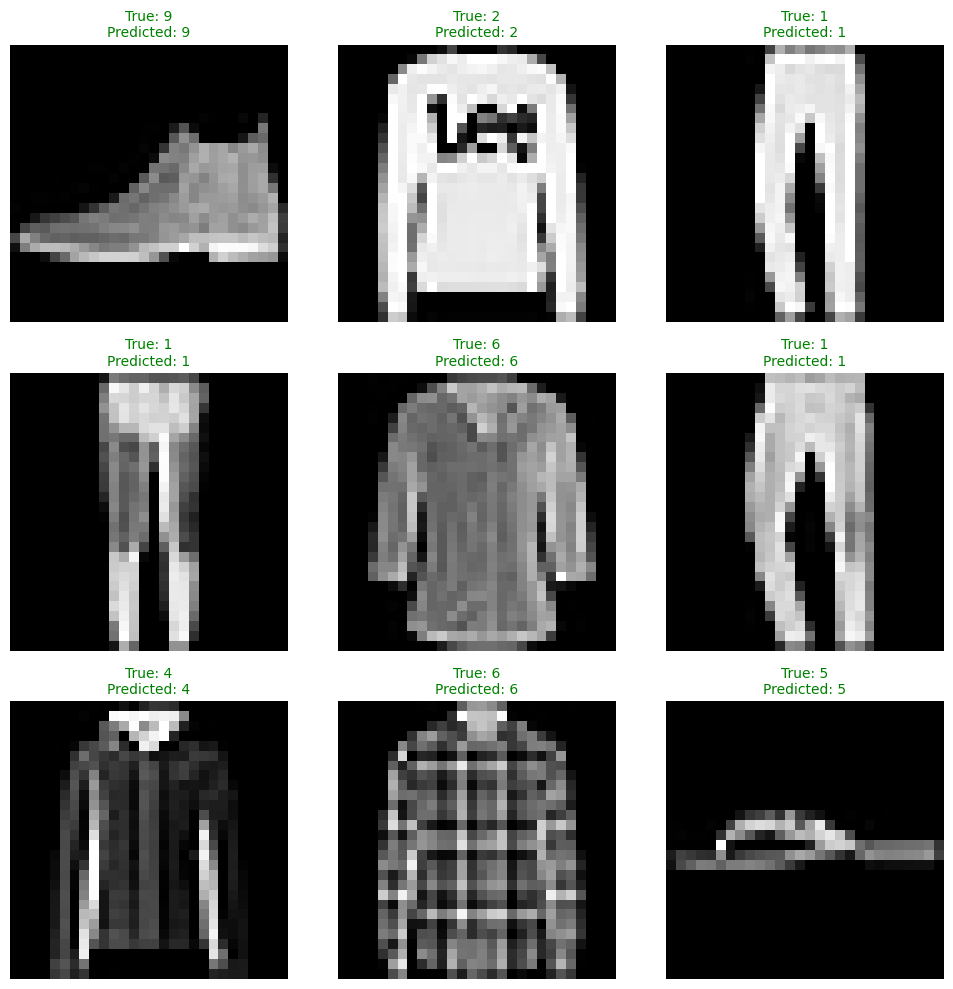
\includegraphics[width=0.8\linewidth]{images/lab1_3_result.png}
\captionof{figure}{Model prediction results}

\justifying

\subsection{Experiment Summary}
During the training process, we used a simple neural network model to train and test the Fashion MNIST dataset. The training process was performed for a total of 25 epochs, with each epoch providing a complete training of the entire training set, and the model performance was evaluated using the test set at the end of each epoch.

\subsubsection{Training Loss and Test Accuracy Change}
The Training Loss (Train Loss) decreases gradually with the increase of epoch number, from about 0.67 initially to about 0.23 eventually.This indicates that the model gradually learns the features and patterns of the data during the training process, and the predictive ability of the model gradually improves as the training progresses.

Test Accuracy (TAR) fluctuated during the training process, but generally showed a gradual improvement. It improves from about 0.80 initially to about 0.87 eventually, which indicates that the model is gradually optimized during the training process and shows better prediction ability for unseen data.
\subsubsection{Experimental Conclusion}

After 25 epochs of training, the model achieves about 87\% accuracy on the test set, which indicates that the simple neural network model achieves better results in handling the Fashion MNIST dataset.
The training loss and test accuracy changes during the training process indicate that the model is gradually optimized during the learning process, but there may be overfitting or fluctuation phenomenon to a certain extent, which can be further improved by adjusting the model architecture, regularization method, or optimizer parameters to further enhance the model performance.

\newpage
\section{Kaggle House Price Prediction}
\subsection{Experimental Purpose}
Design and implement a house price prediction model, train it on the kaggle house price dataset and verify the performance.

\subsection{Experiment Principle}
Use some of the previous basic tools for training deep networks and techniques for network regularization (e.g., weight decay,
temporary recession method, etc.). Put what you've learned into practice through Kaggle competitions. At the same time, there are a few lessons on data preprocessing, model design and hyperparameter selection.
processing, model design and hyperparameter selection.

\subsection{Data Pre-processing}
\subsubsection{Feature Selection}
In the data preprocessing stage, it is first necessary to select the features in the data. Feature selection refers to selecting features from the raw data that are useful for problem solving in order to reduce dimensionality, minimize noise, and improve the efficiency of the model. Common feature selection methods include manual selection based on domain knowledge, automatic selection based on statistical metrics such as variance or correlation, and model-based feature selection methods.

\subsubsection{Handling Missing Values}
There are often missing values in the raw data, i.e., the values of certain features are null or unknown. In the data preprocessing process, missing values need to be handled to avoid adverse effects on model training and evaluation. Common methods for dealing with missing values include deleting samples containing missing values, filling missing values with mean or median values, and using interpolation to fill missing values.

\subsubsection{Feature Scaling and Normalization}
Feature Scaling and Normalization refers to the scaling of data features to ensure that different features have similar scales and distributions among them, so as to improve the training stability and convergence speed of the model. Common feature normalization methods include Z-score normalization and Min-Max normalization:
\begin{itemize}
\item \textbf{Z-score standardization:}
\end{itemize}
\[X_{std} = \frac{X-\mu}{\sigma}\]
Where.
\begin{itemize}
\item $X$ is the original feature value.
\item $\mu$ is the feature mean.
\item $\sigma$ is the characteristic standard deviation.
\end{itemize}

\begin{itemize}
\item \textbf{Min-Max standardization:}
\end{itemize}
\[ X_{\text{scaled}} = \frac{X - X_{\text{min}}}{X_{\text{max}} - X_{\text{min}}} \]
Where.
\begin{itemize}
    \item \( X_{\text{min}} \) and \( X_{\text{max}} \) are the minimum and maximum values of the feature, respectively.
\end{itemize}

\subsubsection{Categorical Data Encoding}
When dealing with data containing categorical variables, categorical features need to be converted into a numerical form that can be understood by the model. Common methods for encoding categorical data include One-Hot Encoding and Label Encoding. One-Hot Encoding expands each categorical variable into multiple binary features that are used to represent each possible category.

\subsection{Cross Validation and Parameter Selection}
K-fold cross-validation helps in model selection and hyperparameter tuning. We first need to define a function that in the
K-fold cross-validation process returns the $i$th fold of data. It selects the $i$th slice as validation data and the remaining
sections as training data. On different cross-validation machines, we can accordingly make the model hyperparameter
selection so as to achieve the optimal result.

\subsection{Experimental Content}
\subsubsection{Data Pre-processing}
\begin{lstlisting}
import pandas as pd
from sklearn.model_selection import train_test_split
from sklearn.preprocessing import StandardScaler, OneHotEncoder
from sklearn.compose import ColumnTransformer
from sklearn.pipeline import Pipeline
from sklearn.impute import SimpleImputer

# 加载训练和测试数据集
train_data_path = 'kaggle_house_pred_train.csv'
test_data_path = 'kaggle_house_pred_test.csv'
train_data = pd.read_csv(train_data_path)
test_data = pd.read_csv(test_data_path)

# 分离特征和目标变量
X_train = train_data.drop('SalePrice', axis=1)  # 特征
y_train = train_data['SalePrice']               # 目标变量

X_test = test_data.copy()  # 测试集没有 'SalePrice' 列

# 选择数值和分类列
numeric_features = X_train.select_dtypes(include=['int64', 'float64']).columns
categorical_features = X_train.select_dtypes(include=['object']).columns

# 创建数值和分类特征的预处理步骤
numeric_transformer = Pipeline(steps=[
    ('imputer', SimpleImputer(strategy='median')),
    ('scaler', StandardScaler())])

categorical_transformer = Pipeline(steps=[
    ('imputer', SimpleImputer(strategy='constant', fill_value='missing')),
    ('onehot', OneHotEncoder(handle_unknown='ignore'))])

# 预处理列并构建ColumnTransformer
preprocessor = ColumnTransformer(
    transformers=[
        ('num', numeric_transformer, numeric_features),
        ('cat', categorical_transformer, categorical_features)])

# 在训练集上拟合预处理器并转换训练集和测试集
X_train = preprocessor.fit_transform(X_train)
X_test = preprocessor.transform(X_test)
\end{lstlisting}

\subsubsection{Model Definition and Training Section}
\begin{lstlisting}
import torch
import torch.nn as nn
import torch.optim as optim
import numpy as np

# 获取输入特征的数量
input_features = X_train.shape[1]

# 定义神经网络模型
class NeuralNetwork(nn.Module):
    def __init__(self, input_features):
        super(NeuralNetwork, self).__init__()
        self.layer1 = nn.Linear(input_features, 64)
        self.layer2 = nn.Linear(64, 32)
        self.layer3 = nn.Linear(32, 1)
        self.relu = nn.ReLU()
    
    def forward(self, x):
        x = self.relu(self.layer1(x))
        x = self.relu(self.layer2(x))
        x = self.layer3(x)
        return x

# 实例化模型
model = NeuralNetwork(input_features)

# 定义损失函数和优化器
criterion = nn.HuberLoss()
optimizer = optim.Adam(model.parameters(), lr=0.001)

# 转换数据为PyTorch张量并进行训练
epochs = 100
for epoch in range(epochs):
    model.train()  # 设置模型为训练模式
    for inputs, targets in train_loader:
        optimizer.zero_grad()
        outputs = model(inputs)
        loss = criterion(outputs, targets)
        loss.backward()
        optimizer.step()
    print(f'Epoch {epoch+1}/{epochs}, Loss: {loss.item()}')

\end{lstlisting}

\subsubsection{Data Forecasting and Submission of Results}
\begin{lstlisting}
# 使用训练好的模型进行预测
model.eval()  # 设置模型为评估模式
with torch.no_grad():
    predictions = model(torch.tensor(X_test, dtype=torch.float32))

# 将预测结果转换为Numpy数组
predictions = predictions.numpy().flatten()

# 假设 'scaler_y' 是用于标准化 'SalePrice' 的 StandardScaler 实例
# 将预测的价格进行逆变换,以转换回原始的价格范围
predicted_prices = scaler_y.inverse_transform(predictions.reshape(-1, 1)).flatten()

# 创建提交DataFrame
submission = pd.DataFrame({
    'Id': test_data['Id'],
    'SalePrice': predicted_prices
})

# 将提交数据保存到CSV文件
submission.to_csv('house_prices_submission.csv', index=False)
\end{lstlisting}

\subsection{Results}
After 100 epochs of training, we can get the following loss variation:
\begin{lstlisting}
Epoch 1/100, Loss: 0.23214686953503152
Epoch 2/100, Loss: 0.08894464956677478
Epoch 3/100, Loss: 0.05397744549681311
Epoch 4/100, Loss: 0.044196434238034744
Epoch 5/100, Loss: 0.04002380893444237
Epoch 6/100, Loss: 0.04059085083882446
Epoch 7/100, Loss: 0.035432298141329185
Epoch 8/100, Loss: 0.034608452742838344
Epoch 9/100, Loss: 0.031963885275889996
Epoch 10/100, Loss: 0.03108540294772905
Epoch 11/100, Loss: 0.02932391712523025
Epoch 12/100, Loss: 0.02814368168701944
Epoch 13/100, Loss: 0.026305337881912357
Epoch 14/100, Loss: 0.02491254865637292
...
Epoch 97/100, Loss: 0.001962528832297286
Epoch 98/100, Loss: 0.0015387779542083001
Epoch 99/100, Loss: 0.0010882699887430215
Epoch 100/100, Loss: 0.0009552285545910506
\end{lstlisting}
The loss variation for training is shown below:

% 去掉figure环境,直接插入图像
\centering % 如果需要居中对齐图像
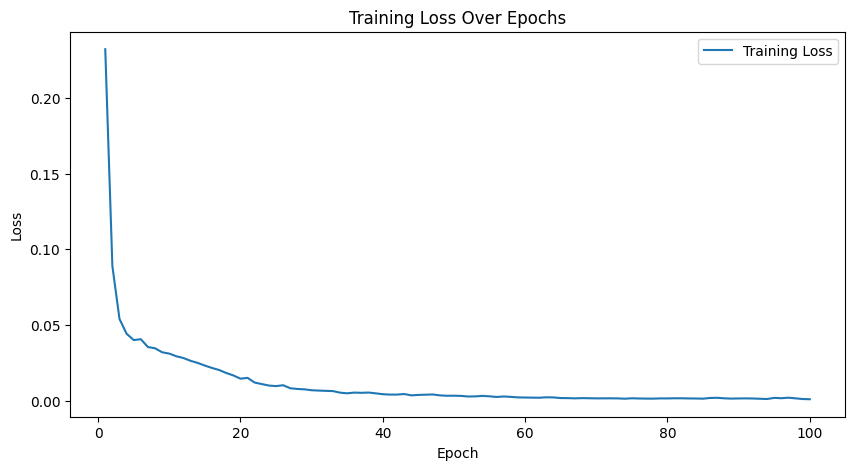
\includegraphics[width=0.8\linewidth]{images/lab1_4_loss.png}
\captionof{figure}{Training loss value} % 使用\captionof命令添加标题
\justifying






\subsection{Experiment Summary}
In the task of house price prediction, model training and evaluation is a key process. The training process of neural network model is analyzed and summarized through the above experiment. In this experiment, we used Huber Loss as the loss function, and by training the preprocessed data, we gradually reduced the loss value of the model from the initial 0.2321 to the final 0.00096. This reduction in the loss value indicates that the model gradually converges during the training process, and learns the patterns and features in the data.

The advantage of using Huber Loss is that it is more robust to outliers. Compared with the traditional Mean Squared Error (MSE) loss function, Huber Loss is able to reduce the impact of outliers on the model training, and improve the stability and generalization of the model. In the task of house price prediction, the house price may be affected by various factors, such as geographic location, house size, surrounding environment, etc., and Huber Loss can better deal with the outliers in these factors, making the model more reliable.

In addition, by observing the change of loss during the training process, we can further adjust the training strategy and hyperparameters of the model to optimize the performance of the model. For example, adjusting the learning rate, choosing a suitable optimizer, etc., to ensure that the model can converge quickly and achieve better results in the training process.

Overall, house price prediction is a complex task that requires comprehensive consideration of multiple factors. Through this experiment, we have gained a deeper understanding of the training process of the neural network model in the task of house price prediction, and provided certain references and ideas for further optimization of the model. Future work will continue to focus on the evaluation and optimization of the model, with the aim of obtaining better prediction results and application performance.

\subsection{Extension Methods}
For the house price prediction experiment, there are other methods such as decision tree regression, random forest regression, LGBM regression, and Adaboost regression. The specific approach is as follows:

\begin{itemize}
    \item Import necessary libraries: This code segment imports the machine learning-related libraries needed, including \texttt{LightGBM}, \texttt{XGBoost}, \texttt{Pandas}, \texttt{NumPy}, \texttt{Scikit-learn}, etc.
    
    \item Custom MAPE function: Defines a function to calculate the Mean Absolute Percentage Error (MAPE).
    
    \item Load the dataset: Loads training and testing data from CSV files.
    
    \item Feature processing: Preprocesses the feature data, including filling and standardizing numerical features, filling and one-hot encoding categorical features, etc.
    
    \item Split the dataset: Divides the dataset into training and testing sets.
    
    \item Define plotting function: Defines a function to visualize the comparison between true and predicted values.
    
    \item Train and predict using different regression models: Trains different regression models such as decision tree regression, random forest regression, \texttt{LightGBM} regression, and \texttt{Adaboost} regression. Then, it makes predictions using the testing set, calculates the Mean Absolute Percentage Error and Mean Absolute Error, and visualizes the comparison between true and predicted values.
\end{itemize} 

This description outlines the process and methodology involved in experimenting with different regression models for house price prediction.

\begin{lstlisting}
import lightgbm as lgb  # 导入整个 lightgbm 库

import xgboost as xgb
# 此处所引入的包大部分为下文机器学习算法
import pandas as pd
from numpy import *
import numpy as np
from sklearn.neural_network import MLPRegressor
from sklearn.tree import DecisionTreeRegressor
from sklearn.ensemble import RandomForestRegressor, AdaBoostRegressor, GradientBoostingRegressor
from sklearn.linear_model import LinearRegression
from sklearn.model_selection import learning_curve
# import xgboost as xgb

from sklearn.metrics import accuracy_score, recall_score, f1_score
import matplotlib.pyplot as plt
from sklearn.metrics import mean_absolute_error
import matplotlib.pyplot as plt
from sklearn.metrics import mean_absolute_error, r2_score
from sklearn.neural_network import MLPRegressor

import warnings

warnings.filterwarnings("ignore")
from sklearn.model_selection import train_test_split
\end{lstlisting}

\begin{lstlisting}
import pandas as pd
from sklearn.model_selection import train_test_split
from sklearn.preprocessing import StandardScaler, OneHotEncoder
from sklearn.compose import ColumnTransformer
from sklearn.pipeline import Pipeline
from sklearn.impute import SimpleImputer
from sklearn.neural_network import MLPRegressor
from sklearn.linear_model import LinearRegression
from sklearn.tree import DecisionTreeRegressor
from sklearn.ensemble import RandomForestRegressor, AdaBoostRegressor
import lightgbm as lgb
from sklearn.metrics import mean_absolute_error, r2_score
import matplotlib.pyplot as plt
import numpy as np

# 自定义MAPE函数
def mape(y_true, y_pred):
    return np.mean(np.abs((y_true - y_pred) / y_true)) * 100

# 加载数据集
train_data_path = 'kaggle_house_pred_train.csv'
test_data_path = 'kaggle_house_pred_test.csv'
train_data = pd.read_csv(train_data_path)
test_data = pd.read_csv(test_data_path)

# 分离特征和目标变量
X = train_data.drop('SalePrice', axis=1)  # 特征
Y = train_data['SalePrice']               # 目标变量

# 选择数值和分类列
numeric_features = X.select_dtypes(include=['int64', 'float64']).columns
categorical_features = X.select_dtypes(include=['object']).columns

# 创建预处理步骤
numeric_transformer = Pipeline(steps=[
    ('imputer', SimpleImputer(strategy='median')),
    ('scaler', StandardScaler())])

categorical_transformer = Pipeline(steps=[
    ('imputer', SimpleImputer(strategy='constant', fill_value='missing')),
    ('onehot', OneHotEncoder(handle_unknown='ignore', sparse_output=False))])

# 预处理列并构建column transformer
preprocessor = ColumnTransformer(
    transformers=[
        ('num', numeric_transformer, numeric_features),
        ('cat', categorical_transformer, categorical_features)])

# 现在将预处理器应用于X和X_test
X_processed = preprocessor.fit_transform(X)
X_test_processed = preprocessor.transform(test_data)

# 拆分数据集
tr_x, te_x, tr_y, te_y = train_test_split(X_processed, Y, test_size=0.3, random_state=5)


def plot_results(true_y, pred_y, title):
    plt.figure(figsize=(10, 6))
    plt.plot(range(true_y.shape[0]), true_y, color='orange', linestyle='--', label='True value', alpha=0.7)
    plt.plot(range(pred_y.shape[0]), pred_y, color='red', linestyle='-', label='Predicted value', alpha=0.7)
    plt.title(title)
    plt.xlabel('Sample Number')
    plt.ylabel('Sale Price')
    plt.legend()
    plt.grid(True, linestyle='--', alpha=0.5)
    plt.show()


# 决策树回归
tree = DecisionTreeRegressor(max_depth=50, random_state=0)
tree.fit(tr_x, tr_y)
y_pred = tree.predict(te_x)
print("\n决策树回归:")
print("训练集平均绝对百分比误差:{:.3f}".format(mape(tree.predict(tr_x), tr_y)))
print("测试集平均绝对百分比误差:{:.3f}".format(mape(tree.predict(te_x), te_y)))
print("平均绝对误差:", mean_absolute_error(te_y, y_pred))
print("r2_score", r2_score(te_y, y_pred))
plot_results(te_y, y_pred, 'Decision Tree Regressor - True vs. Predict')

# 随机森林回归
rf = RandomForestRegressor(random_state=5)
rf.fit(tr_x, tr_y)
y_pred = rf.predict(te_x)
print("\n随机森林回归:")
print("训练集平均绝对百分比误差:{:.3f}".format(mape(rf.predict(tr_x), tr_y)))
print("测试集平均绝对百分比误差:{:.3f}".format(mape(rf.predict(te_x), te_y)))
print("平均绝对误差:", mean_absolute_error(te_y, y_pred))
print("r2_score", r2_score(te_y, y_pred))
plot_results(te_y, y_pred, 'Random Forest Regressor - True vs. Predict')

# LGBM回归
lgb_model = lgb.LGBMRegressor(random_state=5)
lgb_model.fit(tr_x, tr_y)
y_pred = lgb_model.predict(te_x)
print("\nLGBM回归:")
print("训练集平均绝对百分比误差:{:.3f}".format(mape(lgb_model.predict(tr_x), tr_y)))
print("测试集平均绝对百分比误差:{:.3f}".format(mape(lgb_model.predict(te_x), te_y)))
print("平均绝对误差:", mean_absolute_error(te_y, y_pred))
print("r2_score", r2_score(te_y, y_pred))
plot_results(te_y, y_pred, 'LGBM Regressor - True vs. Predict')

# Adaboost回归
ada_model = AdaBoostRegressor(n_estimators=100, random_state=5)
ada_model.fit(tr_x, tr_y)
y_pred = ada_model.predict(te_x)
print("\nAdaboost回归:")
print("训练集平均绝对百分比误差:{:.3f}".format(mape(ada_model.predict(tr_x), tr_y)))
print("测试集平均绝对百分比误差:{:.3f}".format(mape(ada_model.predict(te_x), te_y)))
print("平均绝对误差:", mean_absolute_error(te_y, y_pred))
print("r2_score", r2_score(te_y, y_pred))
plot_results(te_y, y_pred, 'Adaboost Regressor - True vs. Predict')

\end{lstlisting}

\subsubsection{Experimental Results}
The following results can be obtained:

\begin{figure}[H]
    \centering
    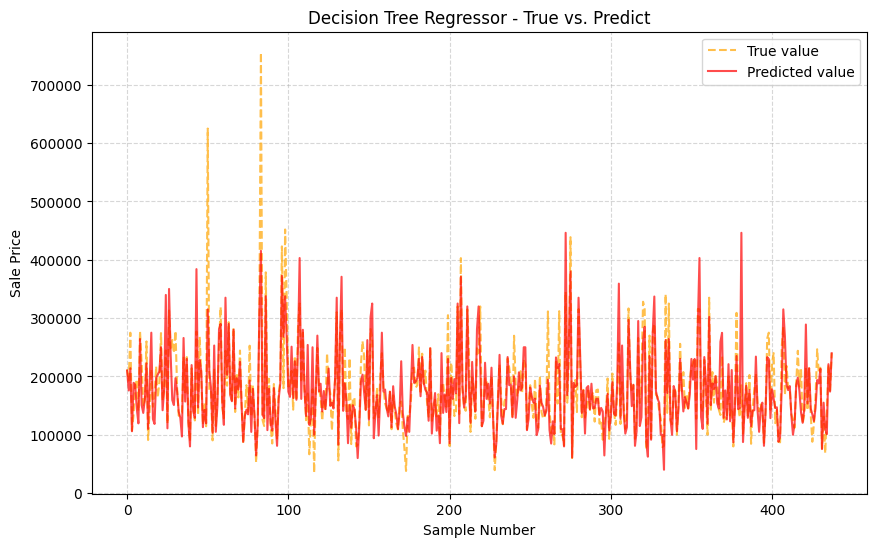
\includegraphics[width=0.75\linewidth]{images/kaggle_DecisionTree.png}
    \caption{Decision Tree Regression Prediction Results}
\end{figure}

\begin{lstlisting}
Decision Tree Regression:
Training set Mean Absolute Percentage Error: 0.000
Testing set Mean Absolute Percentage Error: 15.056
Mean Absolute Error: 26470.70091324201
r2_score: 0.6797460239212758
\end{lstlisting}

\begin{figure}[H]
    \centering
    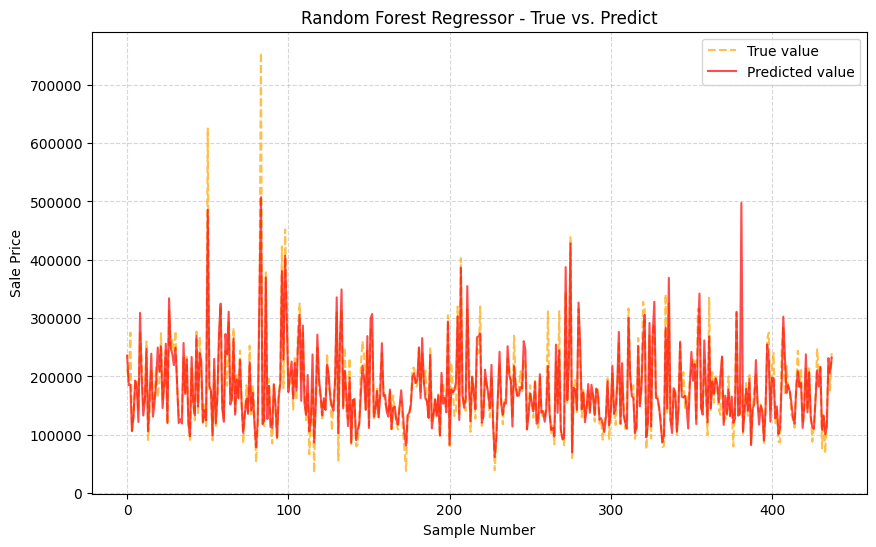
\includegraphics[width=0.75\linewidth]{images/kaggle_RandomForests.png}
    \caption{Random Forest Regression Prediction Results}
\end{figure}

\begin{lstlisting}
Random Forest Regression:
Training set Mean Absolute Percentage Error: 3.729
Testing set Mean Absolute Percentage Error: 9.697
Mean Absolute Error: 17748.21392694064
r2_score: 0.8413617743065108
\end{lstlisting}

\begin{figure}[H]
    \centering
    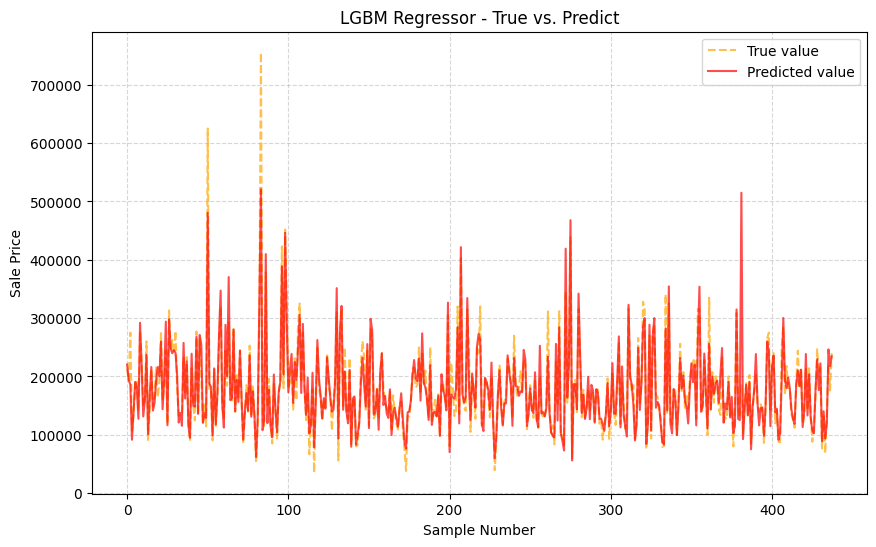
\includegraphics[width=0.75\linewidth]{images/kaggle_LGBM.png}
    \caption{LGBM Regression Prediction Results}
\end{figure}

\begin{lstlisting}
LGBM Regression:
Training set Mean Absolute Percentage Error: 2.605
Testing set Mean Absolute Percentage Error: 9.008
Mean Absolute Error: 16387.722059327447
r2_score: 0.8516765304026097
\end{lstlisting}

\begin{figure}[H]
    \centering
    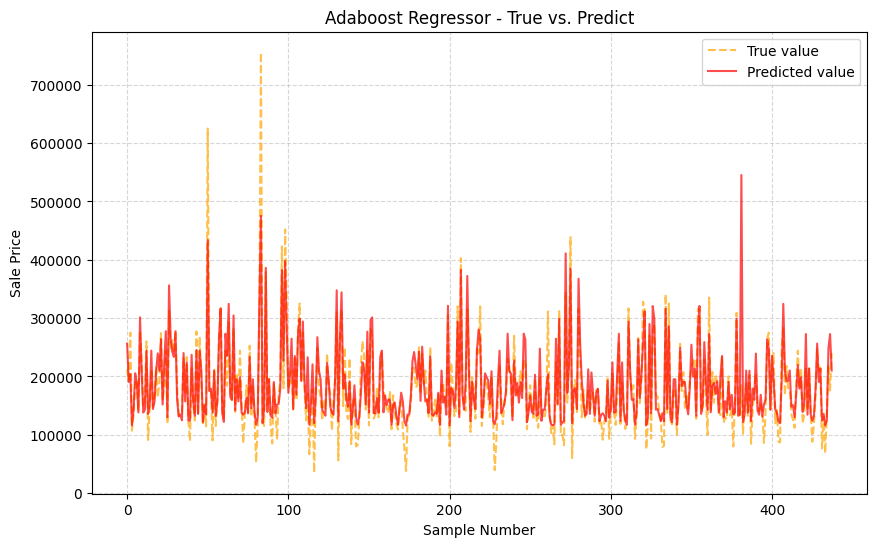
\includegraphics[width=0.75\linewidth]{images/kaggle_Adaboost.png}
    \caption{Adaboost Regression Prediction Results}
\end{figure}

\begin{lstlisting}
Adaboost Regression:
Training set Mean Absolute Percentage Error: 11.846
Testing set Mean Absolute Percentage Error: 12.476
Mean Absolute Error: 23103.15095517458
r2_score: 0.7659513040181836
\end{lstlisting}

\newpage
\section{Convolutional edge detection}
\subsection{Experimental Purpose}
Input an image and design a convolution kernel to detect horizontal edges, vertical edges and diagonal edges in the image and output the results.
\subsection{Experimental Principle}
Convolution is a mathematical operation used to combine two functions to produce a third function. In image processing
convolution is used to apply a filter or convolution kernel to an image to perform operations such as blurring, sharpening or edge detection.
In edge detection, we use convolution to highlight regions of the image that strongly vary in brightness. The basic idea is
Convolution of an image with a convolution kernel that emphasizes regions of significant intensity variation, which correspond to edges.
The convolution operation can be represented by the following mathematical expression:

\begin{equation}
\text{output}(x, y) = \sum_{i, j} \text{kernel}(i, j) \cdot \text{input}(x - i, y - j)
\end{equation}

where:
$output(x, y)$ denotes the output pixel value at position $(x, y)$ in the resultant image. $kernel(i, j)$ refers to the value of the
coefficients of the convolution kernel at position $(i, j)$. $input(x-i, y-j)$ denotes the input pixel value at position $(x-i, y-j)$ in the original image.
at position $(x-i, y-j)$ in the original image. The summation is performed at all positions $(i, j)$ of the convolution kernel. In order to detect different types of
of edges (horizontal, vertical, and diagonal), we need to design specific convolution kernels to capture these directions. The
following are the convolutional kernels used in this experiment:
\begin{itemize}
  \item Horizontal edge detection kernel:
  \[
  \begin{bmatrix}
    -1 & -1 & -1 \\
     2 &  2 &  2 \\
    -1 & -1 & -1
  \end{bmatrix}
  \]
  This kernel is used to detect horizontal edges by enhancing the edges in the horizontal direction of the image. It will enhance the edge strength in the vertical direction and weaken the edge strength in the horizontal direction.

  \item Vertical edge detection kernel:
  \[
  \begin{bmatrix}
    -1 &  2 & -1 \\
    -1 &  2 & -1 \\
    -1 &  2 & -1
  \end{bmatrix}
  \]
  This kernel is used to detect vertical edges by enhancing the edges in the vertical direction of the image.It will weaken the intensity of the edges in the horizontal direction, while the intensity of the edges in the vertical direction will be enhanced.

  \item Diagonal Edge Detection Kernel:
  \[
  \begin{bmatrix}
     2 & -1 & -1 \\
    -1 &  2 & -1 \\
    -1 & -1 &  2
  \end{bmatrix}
  \]
  
  This kernel is used to detect diagonal edges by enhancing the edges in the diagonal direction of the image.It will weaken the strength of edges in horizontal and vertical directions, while the strength of edges on the diagonal will be enhanced.
  
\end{itemize}

\subsection{Experimental Content}
\subsubsection{Data loading and Pre-processing}
\begin{lstlisting}
import torch
import torchvision
from torchvision import transforms
import matplotlib.pyplot as plt

# 定义显示图像的函数
def plot_show(x):
    _, figs = plt.subplots(1, 1, figsize=(5, 5))
    figs.imshow(x.reshape((28, 28)).detach().cpu().numpy(), cmap='gray')
    ax = figs.axes
    ax.get_xaxis().set_visible(False)
    ax.get_yaxis().set_visible(False)
    plt.show()

# 定义数据预处理操作,将数据转换为tensor
transform = transforms.Compose([
    transforms.ToTensor()
])

# 加载 FashionMNIST 数据集并应用预处理操作
fashionMNIST_train = torchvision.datasets.FashionMNIST(root='./data', train=True, download=True, transform=transform)
\end{lstlisting}

\subsubsection{Image Display Functions}
\begin{lstlisting}
# 显示图像的函数
def plot_show(x):
    _, figs = plt.subplots(1, 1, figsize=(5, 5))
    figs.imshow(x.reshape((28, 28)).detach().cpu().numpy(), cmap='gray')
    ax = figs.axes
    ax.get_xaxis().set_visible(False)
    ax.get_yaxis().set_visible(False)
    plt.show()

\end{lstlisting}

\subsubsection{Definition of Convolution Operation}
\begin{lstlisting}
import torch.nn.functional as F

# 定义二维卷积操作函数
def corr2d(X, K):
    # 增加批量大小和通道数维度
    X = X.unsqueeze(0).unsqueeze(0)
    K = K.unsqueeze(0).unsqueeze(0)
    Y = F.conv2d(X, K, padding=1)
    return Y.squeeze()  # 移除多余的维度
\end{lstlisting}

\subsubsection{Results of different convolutional kernel operations}
\begin{lstlisting}
# 获取第一个图像的第一个通道
X = images[0][0]

# 定义不同的卷积核
K_vertical = torch.tensor([[1, 0, -1], [1, 0, -1], [1, 0, -1]], dtype=torch.float32)
Y_vertical = corr2d(X, K_vertical)
plot_show(Y_vertical)

K_horizontal = torch.tensor([[1, 1, 1], [0, 0, 0], [-1, -1, -1]], dtype=torch.float32)
Y_horizontal = corr2d(X, K_horizontal)
plot_show(Y_horizontal)

K_diagonal = torch.tensor([[0, 1, 0], [1, -4, 1], [0, 1, 0]], dtype=torch.float32)
Y_diagonal = corr2d(X, K_diagonal)
plot_show(Y_diagonal)
\end{lstlisting}

\subsection{Results}
The code is detected on Fashion MNIST dataset images and the following results are shown for different convolutional kernels:

% 去掉figure环境,直接插入图像
\centering % 如果需要居中对齐图像
\begin{figure}[htbp]  % 设置浮动环境
    \centering
    % 第一行:原图和竖直检测结果
    \begin{minipage}{0.45\textwidth}
        \centering
        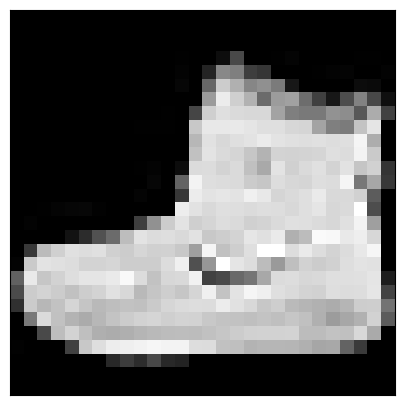
\includegraphics[width=\linewidth]{images/lab2_1_ori.png}
        \caption*{Original figure}
    \end{minipage}
    \hspace{0.05\textwidth}  % 增加水平间距
    \begin{minipage}{0.45\textwidth}
        \centering
        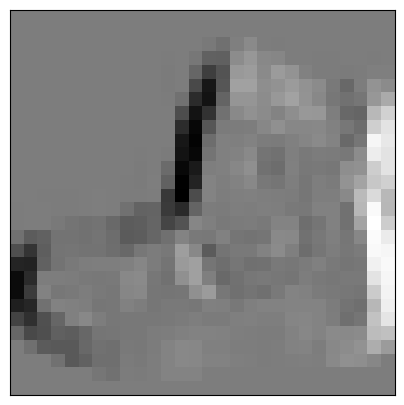
\includegraphics[width=\linewidth]{images/lab2_1_ver.png}
        \caption*{Vertical test results}
    \end{minipage}

    \vspace{1em}  % 增加垂直间距

    % 第二行:水平检测结果和对角线检测结果
    \begin{minipage}{0.45\textwidth}
        \centering
        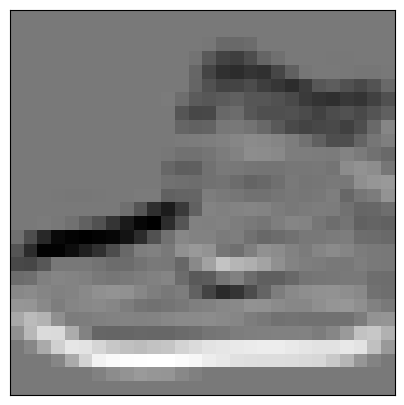
\includegraphics[width=\linewidth]{images/lab2_1_hori.png}
        \caption*{Level detection results}
    \end{minipage}
    \hspace{0.05\textwidth}  % 增加水平间距
    \begin{minipage}{0.45\textwidth}
        \centering
        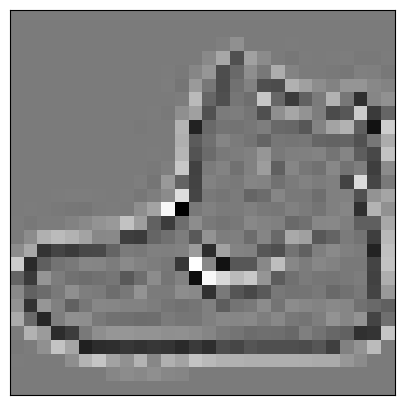
\includegraphics[width=\linewidth]{images/lab2_1_diag.png}
        \caption*{Diagonal test results}
    \end{minipage}

    \caption{Image processing results}  % 整体标题
\end{figure}
\justifying

\newpage
\section{Filling and Pacing}
\subsection{Experimental Purpose}
Design three different sets of fill and step combinations to calculate the output shape using the shape calculation formula and experimentally verify if the results are consistent.

\subsection{Experimental Principle}
\subsubsection{Fill}
When applying multilayer convolution, we often lose edge pixels. Since we usually use a small convolution kernel, due to the fact that
so for any single convolution, we may only lose a few pixels. However, as we apply many consecutive convolutional layers, the cumulative number of pixels lost
layers, the cumulative number of pixels lost is much higher. A simple solution to this problem is padding:
This is done by padding the boundaries of the input image with elements (usually the padding element is 0). If we add $p_h$ rows of padding (about
half at the top and half at the bottom) and $p_w$ column padding (about half on the left and half on the right), the output shape
will be:
\begin{equation}
(n_h - k_h + p_h + 1) \times (n_w - k_w + p_w + 1)
\end{equation}
This means that the height and width of the output will be increased by $p_h $ and $p_w$ respectively. In many cases, we need to set
$p_h = k_h - 1$ and $p_w = k_w - 1$ so that the input and output have the same height and width. This makes it easier to construct the
network more easily by predicting the shape of the output for each layer. Assuming that $k_h$ is odd, we will fill both sides of the height
sides of the height, we will fill the $p_h/2$ rows. If $k_h$ is even, one possibility is to fill $\lceil p_h/2 \rceil$ lines at the top of the input and $\lfloor$ lines at the bottom.
bottom populated with $\lfloor p_h/2 \rfloor$ lines.
The height and width of the convolutional kernel in a convolutional neural network is usually an odd number, such as 1, 3, 5, or 7.
number has the advantage of maintaining the spatial dimensionality while allowing us to populate the same number of rows on the top and bottom, and the same number of rows on the
the top and bottom, and the same number of columns on the left and right.

\subsubsection{Pace}
When calculating mutual correlations, the convolution window starts at the top left corner of the input tensor and slides down and to the right. In many
cases, we default to sliding one element at a time. However, in some cases, for efficient computation or to minimize the number of samples, the convolution window can skip the middle of the
or to reduce the number of samples, the convolution window can skip the center and slide more than one element at a time. Typically, when the vertical step size is $s_h$, the horizontal step size is $s_w$, and the horizontal step size is $s_w$.
When the vertical step is $s_h$ and the horizontal step is $s_w$, the output shape is

\begin{equation}
\left\lfloor \frac{nh - kh + ph + sh}{sh} \right\rfloor \times \left\lfloor \frac{nw - kw + pw + sw}{sw} \right\rfloor
\end{equation}
If we set \( p_h = k_h - 1 \) and \( p_w = k_w - 1 \), the output shape simplifies to \( \left\lfloor (n_h + s_h - 1)/s_h \right\rfloor \times \left\lfloor (n_w + s_w - 1)/s_w \right\rfloor \). In addition, if the height and width of the input can be divided by the vertical and horizontal steps, then the output shape will be \( n_h/s_h \times n_w/s_w \).

\subsection{Experimental Content}
The output shape of the convolutional layer is calculated as follows:
Output Shape = ((Input Shape - Convolution Kernel Size + 2 * Fill) / Step) + 1
\subsubsection{Programming for three sets of fill and step operations}
\begin{lstlisting}
def calculate_output_shape(input_shape, kernel_size, padding, stride):
    # 计算输出形状
    output_shape = ((input_shape - kernel_size + 2 * padding) // stride) + 1
    return output_shape

# 组合1
input_shape = 32
kernel_size = 3
padding = 1
stride = 1

# 调用函数计算输出形状
output_shape = calculate_output_shape(input_shape, kernel_size, padding, stride)
print("组合1:")
print("输出形状:", output_shape)

# 组合2
input_shape = 64
kernel_size = 5
padding = 2
stride = 2

# 调用函数计算输出形状
output_shape = calculate_output_shape(input_shape, kernel_size, padding, stride)
print("\n组合2:")
print("输出形状:", output_shape)

# 组合3
input_shape = 28
kernel_size = 3
padding = 0
stride = 2

# 调用函数计算输出形状
output_shape = calculate_output_shape(input_shape, kernel_size, padding, stride)
print("\n组合3:")
print("输出形状:", output_shape)
\end{lstlisting}
Output results:
\begin{lstlisting}
组合1:
输出形状: 32
组合2:
输出形状: 32
组合3:
输出形状: 13
\end{lstlisting}

\subsubsection{Results and Verification}
Here are the combinations enclosed in the itemize environment:

\begin{itemize}
  \item Combination 1:
  \begin{align*}
  \text{Input shape:} & 32 \\
  \text{Kernel size:} & 3 \\
  \text{Padding:} & 1 \\
  \text{Stride:} & 1 \\
  \text{Output shape} & = \left( \frac{32 - 3 + 2 \times 1}{1} \right) + 1 = 32
  \end{align*}

  \item Combination 2:
  \begin{align*}
  \text{Input shape:} & 64 \\
  \text{Kernel size:} & 5 \\
  \text{Padding:} & 2 \\
  \text{Stride:} & 2 \\
  \text{Output shape} & = \left( \frac{64 - 5 + 2 \times 2}{2} \right) + 1 = 32
  \end{align*}

  \item Combination 3:
  \begin{align*}
  \text{Input shape:} & 28 \\
  \text{Kernel size:} & 3 \\
  \text{Padding:} & 0 \\
  \text{Stride:} & 2 \\
  \text{Output shape} & = \left( \frac{28 - 3 + 2 \times 0}{2} \right) + 1 = 13
  \end{align*}
\end{itemize}

\subsection{Results}
Both the results obtained by the code and the manual calculations are consistent.

\subsection{Experiment Summary}
In this experiment, we tried different combinations of input shape, convolution kernel size, padding and step size parameters and observed their effects on the output shape.

First, in combination 1, we set the input shape to 32, the convolution kernel size to 3, the padding to 1, and the step size to 1. The results show that the output shape after the convolution operation is the same as the input shape, which indicates that the convolution operation does not change the size of the feature map under this setting.

Second, in Combination 2, we set the input shape to 64, the convolution kernel size to 5, the fill to 2, and the step size to 2. The result shows that the output shape is reduced to 32 after the convolution operation, which indicates that we can control the size of the feature map with this setting.

Finally, in combination 3, we set the input shape as 28, the convolution kernel size as 3, the fill as 0, and the step size as 2. The result shows that the output shape after convolution operation is 13, and the setting of the step size affects the scaling ratio of the output shape, which is important for resizing the feature map and extracting the image features.

In summary, the parameter settings in the convolution operation have a significant impact on the performance of the neural network and feature extraction. By adjusting the parameters such as input shape, convolution kernel size, padding and step size, we can flexibly control the output shape of the convolution operation, thus realizing effective processing of image data and feature extraction.

\newpage
\section{1*1 convolution Kernel}
\subsection{Experimental Purpose}
To adjust the number of channels between network layers using a 1*1 convolution kernel so that the number of channels is halved.

\subsection{Experimental Principle}
A $1 \times 1$ convolution kernel, also known as point-by-point convolution or network-within-a-network operation, is a convolution kernel with spatial scale
convolution kernel with a $1 \times 1$ dimension. Unlike larger convolution kernel sizes, a $1x1$ convolution kernel does not capture the spatial relationship between neighboring pixels, but instead focuses on changing the
neighboring pixels, but rather focuses on changing the channel representation of the input feature map.

To understand the formula for the $1 \times 1$ convolution, let us consider the input feature map tensor of shape $(C, H, W)$, where $C $ denotes the channel representation of the input channel.
where $C $ denotes the number of input channels, and $H $ and $W $ denote the height and width of the feature map, respectively. Each element of the feature map
Each element in the feature map can be represented as $x(c, h, w)$, where $c $ ranges from $0$ to $C-1$, $h $ ranges from $0$ to $H-1$, and $w $ ranges from $0$ to $H-1$.
$w $ ranges from $0 $ to $W-1$.

The $1 \times 1$ convolution applies a set of learnable filters (also called convolution kernels or weights) to the input feature map.
These filters are of size $1x1$ and have the same number of channels as the input feature map. Let us denote the $1 \times 1$ convolutional
weight tensor of the product as $W(c', c)$, where $c' $ ranges from 0 to $C'-1$, and $C'$ denotes the number of output channels
The output channel number is denoted by $C'$.

The output feature map tensor generated by the convolution of $1 \times 1$ has the form of shape $(C', H, W) $, where each of the
element can be represented as $y(c', h, w)$, where c' ranges from 0 to $c'-1$, $h $ ranges from 0 to H-1, and w
ranges from $0 $ to $W-1$.

To compute the output feature map, the $1x1 $ convolution applies the following equation:
\begin{equation}
y(c', h, w) = \sum_{c=0} x(c, h, w) \cdot W(c', c)
\end{equation}
In this formulation, the output feature map element $y(c', h, w)$ is computed by summing the input feature map $x(c, h, w)$ and the
the element-by-element product between the corresponding weights $W(c', c)$. The summation is performed on all input channels from $c=0$
to $C-1$.

The $1 \times 1$ convolution operation is usually followed by a nonlinear activation function (e.g., ReLU) to introduce nonlinearity into the network.
The activation function is applied element by element to each element in the output feature map.

The $1 \times 1$ convolution allows for dimensionality reduction or expansion by modifying the number of channels, while maintaining the input feature map's
the spatial dimension of the input feature map. It is often used in deep neural networks to adjust the number of channels and control the complexity of the model.

The figure below shows a correlation calculation using a $1 \times 1$ convolution kernel with 3 input channels and 2 output channels.
The following figure shows the inter-correlation calculation using a $1 \times 1$ convolution kernel with 3 input channels and 2 output channels. Here the inputs and outputs have the same height and width, and each element in the output is a linear representation of an element at the same location from the input image.
Each element in the output is a linear combination of elements from the same position in the input image. We can think of the $1 \times 1$ convolutional layer as a fully connected layer that is applied at each pixel position.
at each pixel location, converting $c_i$ input values to $c_o$ output values. Since this is still a convolutional layer, the
weights are consistent across pixels.

% 去掉figure环境,直接插入图像
\centering % 如果需要居中对齐图像
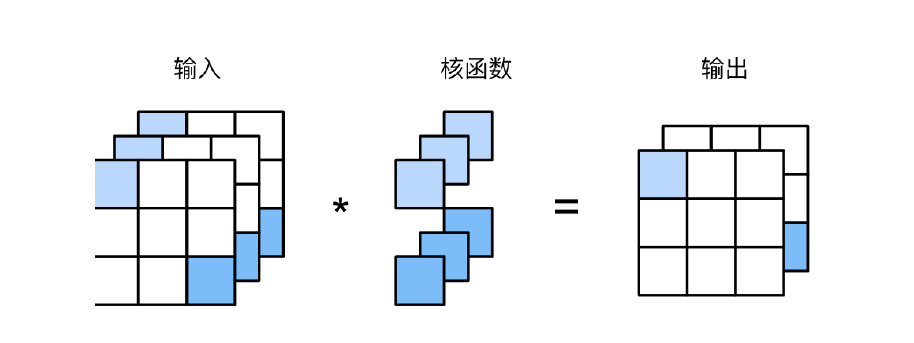
\includegraphics[width=0.8\linewidth]{images/1x1.png}
\captionof{figure}{1$\times $1 Convolution Schematic} % 使用\captionof命令添加标题

\justifying


\subsection{Experimental Content}
\subsubsection{$1 \times 1$ convolution method with multiple inputs and multiple outputs}
Each element in the output is a linear combination of elements from the same position in the input image. One can think of the $1 \times 1$
convolutional layer as a fully connected layer applied at each pixel location to convert $c_i $ input values to $c_o $ output values.
\begin{lstlisting}
def corr2d_multi_in_out_1x1(X, K):
    c_i, h, w = X.shape
    c_o = K.shape[0]
    X = X.reshape((c_i, h * w))
    K = K.reshape((c_o, c_i))
    # 全连接层中的矩阵乘法
    Y = torch.matmul(K, X)
    return Y.reshape((c_o, h, w))

import torch
import torch.nn as nn

X = torch.normal(0, 1, (3, 3, 3))
K = torch.normal(0, 1, (2, 3, 1, 1))
print(X)
print(K)

Y1 = corr2d_multi_in_out_1x1(X, K)
print(X.shape)
print(K.shape)
print(Y1.shape)

\end{lstlisting}
\subsubsection{The $1 \times 1$ convolution method for halving the number of channels}
\begin{lstlisting}
import torch
import torch.nn as nn

# 定义一个具有16个输入通道的样本输入张量,形状为(batch_size, in_channels, height, width)
input_tensor = torch.randn(8, 16, 32, 32)

# 定义一个自定义模块,使用1x1卷积将通道数量减半
class ChannelHalvingModule(nn.Module):
    def __init__(self, in_channels, out_channels):
        super(ChannelHalvingModule, self).__init__()
        self.conv1x1 = nn.Conv2d(in_channels, out_channels, kernel_size=1)

    def forward(self, x):
        return self.conv1x1(x)

# 创建自定义模块的实例
module = ChannelHalvingModule(in_channels=16, out_channels=8)

# 将输入张量传递给模块
output_tensor = module(input_tensor)

# 打印输入张量和输出张量的形状
print("输入张量形状:", input_tensor.shape)
print("输出张量形状:", output_tensor.shape)
\end{lstlisting}

\subsection{Results}
In the multi-input multi-output $1 \times 1$ convolution method, we obtain the following results.
\begin{lstlisting}
torch.Size([3, 3, 3])
torch.Size([2, 3, 1, 1])
torch.Size([2, 3, 3])
\end{lstlisting}
It can be observed that the number of channels has changed from 3 to 2.

In the $1 \times 1$ convolution method with the number of channels halved, we obtain the following results.
\begin{lstlisting}
输入张量形状: torch.Size([8, 16, 32, 32])
输出张量形状: torch.Size([8, 8, 32, 32])
\end{lstlisting}
It can be observed that the number of channels has been halved from 16 to 8.

\subsection{Experimental Summary}
The experimental results show that the use of the $1 \times 1$ convolution kernel allows for an efficient tuning of the number of channels while keeping the spatial size of the feature map constant. This adjustment is important for both the computational efficiency of the model and the number of parameters. By appropriately adjusting the number of channels, we can control the complexity of the model and help to improve the expressive and generalization ability of the model. Therefore, $1 \times 1$convolution kernels in neural networks are widely useful and have important roles in various tasks and model structures.

\newpage
\section{LeNet}
\subsection{Experimental Purpose}
Recognition of MNIST databases using LeNet, testing different convolutional kernel size, padding and step size
combinations on the results.

\subsection{Experimental Principle}
LeNet, which is one of the earliest released convolutional neural networks, has received a lot of attention for its efficient in computer vision task
performance and has received much attention. This model was developed by Yann LeCun, a researcher at AT T Bell Labs, in
1989 (and named after him) with the aim of recognizing images. In general, LeNet (LeNet-5) consists of a
two parts: a convolutional encoder and a dense block of fully connected layers:

\begin{itemize}
    \item Convolutional encoder: consists of two convolutional layers.
    \item Fully Connected Layer Dense Block: consists of three fully connected layers.
\end{itemize}

% 去掉figure环境,直接插入图像
\centering % 如果需要居中对齐图像
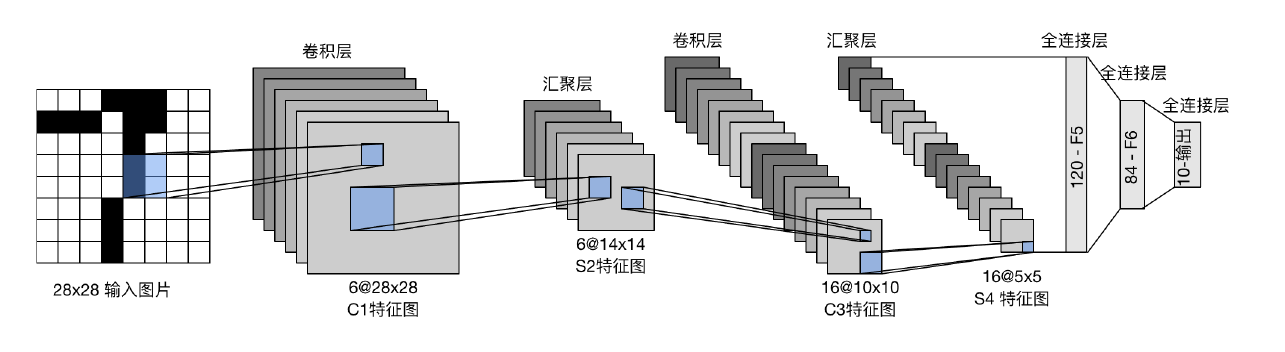
\includegraphics[width=0.8\linewidth]{images/LeNet.png}
\captionof{figure}{Schematic diagram of LeNet structure} % 使用\captionof命令添加标题

\justifying

The basic units in each convolutional block are a convolutional layer, a sigmoid activation function, and an average convergence
layer. Note that although ReLU and maximum convergence layers are more efficient, they were not available in the 1990s.
existed in the 1990s. Each convolutional layer uses a $5 \times 5$ convolutional kernel and a sigmoid activation function. These layers map the input
to multiple 2D feature outputs, often while increasing the number of channels. The first convolutional layer has 6 output channels, while the
The second convolutional layer has 16 output channels. Each $2 \times 2$ pooling operation (step 2) reduces the number of dimensions by a factor of 4 through spatial downsampling.
dimensionality by a factor of 4 through spatial downsampling. The shape of the output of the convolution is determined by the batch size, number of channels, height, and width.

In order to pass the output of the convolution block to the thick block, each sample must be spread in a small batch. In other words.
Convert this four-dimensional input into the two-dimensional input expected by the fully connected layer. The first dimension of the two-dimensional representation here
LeNet's dense block has three fully-connected layers, each of which is a fully-connected layer, and the second dimension gives a planar vector representation of each sample.
The dense block of LeNet has three fully connected layers with 120, 84, and 10 outputs, respectively. Since we are performing a classification task, the
Since we are performing a classification task, the 10 dimensions of the output layers correspond to the number of final outputs.

\subsection{Experimental Content}
\subsubsection{Network Definition}
Contains the Net class that defines the structure of the network, which includes definitions of the convolutional, fully connected, and pooling layers.
\begin{lstlisting}
# Define the network architecture
class Net(nn.Module):
    def __init__(self):
        super(Net, self).__init__()
        self.conv1 = nn.Conv2d(1, 6, kernel_size=5, padding=2)
        self.conv2 = nn.Conv2d(6, 16, kernel_size=5)
        self.fc1 = nn.Linear(16 * 5 * 5, 120)
        self.fc2 = nn.Linear(120, 84)
        self.fc3 = nn.Linear(84, 10)

    def forward(self, x):
        x = torch.sigmoid(self.conv1(x))
        x = nn.functional.avg_pool2d(x, kernel_size=2, stride=2)
        x = torch.sigmoid(self.conv2(x))
        x = nn.functional.avg_pool2d(x, kernel_size=2, stride=2)
        x = torch.flatten(x, 1)
        x = torch.sigmoid(self.fc1(x))
        x = torch.sigmoid(self.fc2(x))
        x = self.fc3(x)
        return x

\end{lstlisting}

\subsubsection{Train Function}
Contains the train function for training the network, which includes training loops, testing network performance, and printing training statistics.
\begin{lstlisting}
# Function to train the network
def train(net, train_loader, test_loader, num_epochs, lr, device):
    criterion = nn.CrossEntropyLoss()
    optimizer = optim.SGD(net.parameters(), lr=lr)

    train_losses, train_accs, test_accs = [], [], []
    for epoch in range(num_epochs):
        net.train()
        running_loss, correct, total = 0.0, 0, 0
        for inputs, labels in train_loader:
            inputs, labels = inputs.to(device), labels.to(device)
            optimizer.zero_grad()
            outputs = net(inputs)
            loss = criterion(outputs, labels)
            loss.backward()
            optimizer.step()
            running_loss += loss.item() * inputs.size(0)
            _, predicted = torch.max(outputs, 1)
            correct += (predicted == labels).sum().item()
            total += labels.size(0)
        train_loss = running_loss / len(train_loader.dataset)
        train_acc = correct / total

        # Test the network
        net.eval()
        correct = 0
        total = 0
        with torch.no_grad():
            for inputs, labels in test_loader:
                inputs, labels = inputs.to(device), labels.to(device)
                outputs = net(inputs)
                _, predicted = torch.max(outputs, 1)
                correct += (predicted == labels).sum().item()
                total += labels.size(0)
        test_acc = correct / total

        # Print statistics
        print(f'Epoch {epoch + 1}/{num_epochs}, '
              f'Train Loss: {train_loss:.4f}, Train Acc: {train_acc:.4f}, '
              f'Test Acc: {test_acc:.4f}')

        train_losses.append(train_loss)
        train_accs.append(train_acc)
        test_accs.append(test_acc)

    return train_losses, train_accs, test_accs
\end{lstlisting}

\subsubsection{Data Preparation and Initialization}
Contains sections for preparing the dataset and initializing the network.
\begin{lstlisting}
# Prepare the data loaders
transform = transforms.Compose([transforms.ToTensor(), transforms.Normalize((0.5,), (0.5,))])
train_loader = torch.utils.data.DataLoader(
    datasets.MNIST(root='./data', train=True, download=True, transform=transform),
    batch_size=64, shuffle=True)
test_loader = torch.utils.data.DataLoader(
    datasets.MNIST(root='./data', train=False, download=True, transform=transform),
    batch_size=1000, shuffle=False)

# Initialize the network
net = Net()
\end{lstlisting}

\subsubsection{Train Network and Plot Curve}
Contains sections for calling the training function, training the network, and plotting the training loss and accuracy curves.
\begin{lstlisting}
# Define training parameters
lr = 0.9
num_epochs = 20
device = torch.device("cuda" if torch.cuda.is_available() else "cpu")

# Move the network to the appropriate device
net.to(device)

# Train the network
train_losses, train_accs, test_accs = train(net, train_loader, test_loader, num_epochs, lr, device)

# Plot the training loss and accuracy
plt.figure(figsize=(10, 4))
plt.subplot(1, 2, 1)
plt.plot(train_losses)
plt.xlabel('Epoch')
plt.ylabel('Train Loss')
plt.title('Training Loss')

plt.subplot(1, 2, 2)
plt.plot(train_accs, label='Train Acc')
plt.plot(test_accs, label='Test Acc')
plt.xlabel('Epoch')
plt.ylabel('Accuracy')
plt.title('Training and Test Accuracy')
plt.legend()
plt.show()

\end{lstlisting}

\subsubsection{Visualize Prediction Results}
Contains the function that visualizes the predicted results of the model and the section that calls the function.
\begin{lstlisting}
# Function to visualize predictions
def visualize_predictions(net, test_loader, device):
    net.eval()
    with torch.no_grad():
        for inputs, labels in test_loader:
            inputs, labels = inputs.to(device), labels.to(device)
            outputs = net(inputs)
            _, predicted = torch.max(outputs, 1)

            # Visualize a batch of predictions
            plt.figure(figsize=(10, 4))
            for i in range(10):
                plt.subplot(2, 5, i + 1)
                plt.imshow(inputs[i].cpu().squeeze().numpy(), cmap='gray')
                plt.title(f'Pred: {predicted[i]}, True: {labels[i]}')
                plt.axis('off')
            plt.tight_layout()
            plt.show()
            break  # Show only one batch of predictions

# Visualize predictions
visualize_predictions(net, test_loader, device)

\end{lstlisting}

\subsection{Results}
After the learning rate is set to 0.9 and 20 epochs of training, the loss is 0.0275, the train acc is 0.9913, and the
test acc is 0.9872. The results are as follows:

\begin{lstlisting}
Epoch 1/20, Train Loss: 2.3087, Train Acc: 0.1044, Test Acc: 0.1135
Epoch 2/20, Train Loss: 2.3048, Train Acc: 0.1055, Test Acc: 0.0982
Epoch 3/20, Train Loss: 2.3044, Train Acc: 0.1072, Test Acc: 0.1009
...
Epoch 18/20, Train Loss: 0.0325, Train Acc: 0.9897, Test Acc: 0.9847
Epoch 19/20, Train Loss: 0.0305, Train Acc: 0.9906, Test Acc: 0.9877
Epoch 20/20, Train Loss: 0.0275, Train Acc: 0.9913, Test Acc: 0.9872
\end{lstlisting}

The LeNet training loss and accuracy varies with epoch as follows

% 去掉figure环境,直接插入图像
\centering % 如果需要居中对齐图像
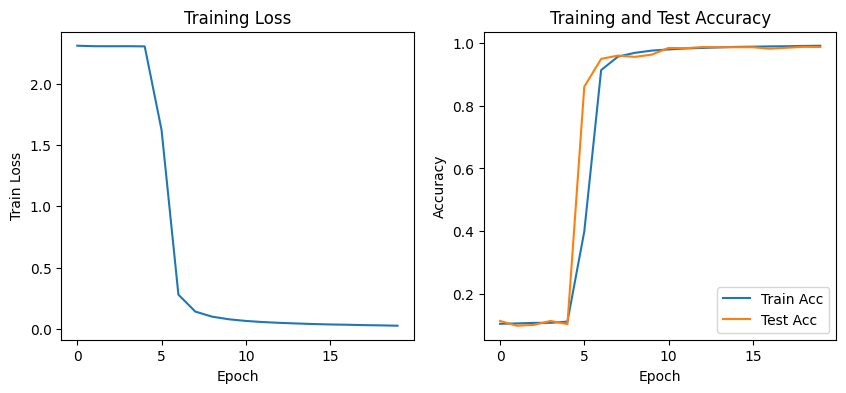
\includegraphics[width=0.8\linewidth]{images/lab2_4_loss.png}
\captionof{figure}{LeNet Training Losses and Precision Values} % 使用\captionof命令添加标题

\justifying

\subsection{Experimental Summary}
By training the LeNet model, we observed the following experimental results:

In the initial phase of training (Epoch 1-5), the training loss and accuracy of the model did not improve significantly, and the test accuracy also remained low. This suggests that the model has a weak learning ability in the initial phase and may require more training cycles to improve performance.

The performance of the model gradually improves as the training progresses. In the subsequent training phases (Epoch 6-20), the training loss and test accuracy of the model show a steady increase. In particular, after Epoch 6, both training loss and test accuracy improved significantly, indicating that the model started to learn effective features and patterns, thus improving its ability to fit the data.

In the final training phase (Epoch 16-20), the training loss of the model gradually stabilizes, while the test accuracy stabilizes at a high level. This indicates that the model achieves good performance on both the training and test sets, has strong generalization ability, and is able to achieve good predictions on unseen data.

Lenet achieves better classification on the MNIST dataset with less training.
Lenet achieves good classification results on the MNIST dataset with little training. Although LeNet is relatively simple, its innovative ideas and some core advantages lay a good foundation for the subsequent development of deep learning.
learning.

\newpage
\section{AlexNet}
\subsection{Experimental Purpose}
To recognize the MNIST database using AlexNet to achieve the optimal recognition rate.

\subsection{Experimental Principle}
In 2012, AlexNet came out of nowhere. It proved for the first time that learned features can outperform hand-designed features.
features. AlexNet uses an 8-layer convolutional neural network, and has a significant advantage over other computer vision research.
AlexNet used an 8-layer convolutional neural network and won the 2012 ImageNet Image Recognition Challenge by a wide margin.

The architectures of AlexNet and LeNet are very similar, as shown in the following figure.

\centering % 如果需要居中对齐图像
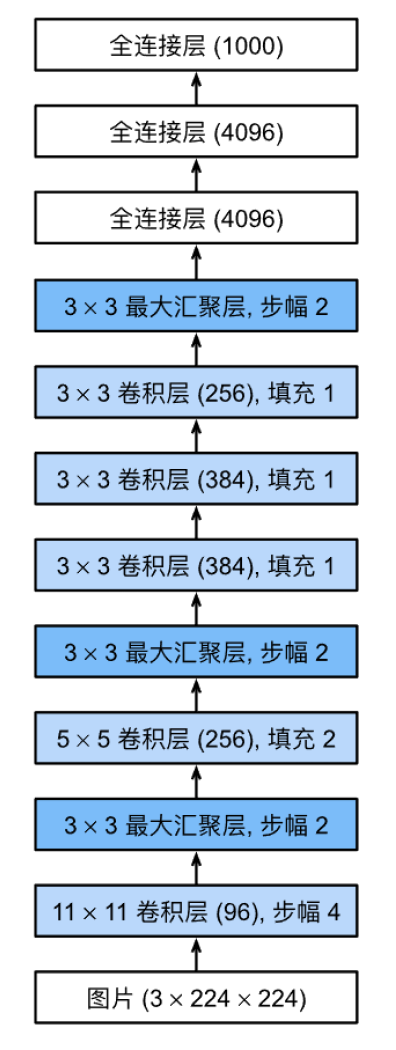
\includegraphics[scale=0.5]{images/AlexNet.png}
\captionof{figure}{Schematic diagram of AlexNet structure} % 使用\captionof命令添加标题
\justifying

The design concepts of AlexNet and LeNet are very similar, but there are significant differences.
\begin{itemize}
    \item AlexNet is much deeper than the relatively small LeNet5. AlexNet consists of eight layers: five convolutional layers,
two fully-connected hidden layers, and one fully-connected output layer.

    \item AlexNet uses ReLU instead of sigmoid as its activation function.
\end{itemize}

In the first layer of AlexNet, the shape of the convolution window is $11 \times 11$. Since most of the ImageNet
images are more than 10 times wider and taller than MNIST images, a larger convolution window is needed to
capture the target. The shape of the convolution window in the second layer is reduced to $5 \times 5$, followed by $3 \times 3$. In addition, in the first
layer, the second and fifth convolutional layers are followed by a maximum convergence layer with a window shape of $3 \times 3$ and a step size of 2.
Moreover, AlexNet has 10 times more convolutional channels than LeNet.

In addition, AlexNet changes the sigmoid activation function to a simpler ReLU activation function. On the one hand, the
On the one hand, the ReLU activation function is simpler to compute, and it does not need the complex power operation as the sigmoid activation function.
The ReLU activation function is simpler to compute. On the other hand, the ReLU activation function makes it easier to train the model when different parameter initialization methods are used.
when different parameter initialization methods are used. When the output of the sigmoid activation function is very close to 0 or 1, the gradient in these regions is almost 0, so backpropagation cannot continue.
When the output of the sigmoid activation function is very close to 0 or 1, the gradient in these regions is almost 0, so backpropagation cannot continue to update some model parameters. On the contrary, the gradient of the ReLU activation function in positive intervals is always 1.
Therefore, if the model parameters are not properly initialized, the sigmoid function may get a gradient of almost 0 in the positive interval, and the backpropagation cannot continue to update some model parameters.
Therefore, if the model parameters are not initialized correctly, the sigmoid function may have a gradient of almost 0 in the positive interval, which prevents the model from being trained efficiently.

AlexNet controls the model complexity of the fully-connected layer by dropout, whereas LeNet uses only weight
decay. To further expand the data, AlexNet adds a large amount of image enhancement data during training, such as flipping, cropping, and color changing.
rotation, cropping, and color change. This makes the model more robust, and the larger sample size effectively reduces overfitting.

\subsection{Experimental Content}
\subsubsection{Network Definition}

\begin{lstlisting}
import torch
import torch.nn as nn
import torch.optim as optim
import torchvision
import torchvision.transforms as transforms
import matplotlib.pyplot as plt

# 定义 AlexNet 模型
class AlexNetFashionMNIST(nn.Module):
    def __init__(self):
        super(AlexNetFashionMNIST, self).__init__()
        self.features = nn.Sequential(
            nn.Conv2d(1, 64, kernel_size=11, stride=4, padding=2),
            nn.ReLU(inplace=True),
            nn.MaxPool2d(kernel_size=3, stride=2),
            nn.Conv2d(64, 192, kernel_size=5, padding=2),
            nn.ReLU(inplace=True),
            nn.MaxPool2d(kernel_size=3, stride=2),
            nn.Conv2d(192, 384, kernel_size=3, padding=1),
            nn.ReLU(inplace=True),
            nn.Conv2d(384, 256, kernel_size=3, padding=1),
            nn.ReLU(inplace=True),
            nn.Conv2d(256, 256, kernel_size=3, padding=1),
            nn.ReLU(inplace=True),
            nn.MaxPool2d(kernel_size=3, stride=2),
        )
        self.avgpool = nn.AdaptiveAvgPool2d((6, 6))
        self.classifier = nn.Sequential(
            nn.Dropout(),
            nn.Linear(256 * 6 * 6, 4096),
            nn.ReLU(inplace=True),
            nn.Dropout(),
            nn.Linear(4096, 4096),
            nn.ReLU(inplace=True),
            nn.Linear(4096, 10),
        )

    def forward(self, x):
        x = self.features(x)
        x = self.avgpool(x)
        x = x.view(x.size(0), 256 * 6 * 6)
        x = self.classifier(x)
        return x

\end{lstlisting}
\subsubsection{Data Preprocessing and Initialization}
\begin{lstlisting}
# 数据预处理
transform = transforms.Compose([
    transforms.Resize((224, 224)),  # 调整图像大小以适应 AlexNet 的输入
    transforms.Grayscale(num_output_channels=1),  # 将图像转换为灰度图像(1个通道)
    transforms.ToTensor(),
    transforms.Normalize((0.5,), (0.5,))
])

# 加载数据集
train_set = torchvision.datasets.FashionMNIST(root='./data', train=True, download=True, transform=transform)
train_loader = torch.utils.data.DataLoader(train_set, batch_size=64, shuffle=True)

\end{lstlisting}

\subsubsection{Training Model}
\begin{lstlisting}
# 创建模型、损失函数和优化器,并将模型加载到 GPU 上
device = torch.device("cuda" if torch.cuda.is_available() else "cpu")
model = AlexNetFashionMNIST().to(device)
criterion = nn.CrossEntropyLoss()
optimizer = optim.Adam(model.parameters(), lr=0.001)

# 训练模型
epochs = 20
train_losses = []
train_accs = []
for epoch in range(epochs):
    running_loss = 0.0
    correct_train = 0
    total_train = 0
    for i, data in enumerate(train_loader, 0):
        inputs, labels = data[0].to(device), data[1].to(device)  # 将数据加载到 GPU 上
        optimizer.zero_grad()
        outputs = model(inputs)
        loss = criterion(outputs, labels)
        loss.backward()
        optimizer.step()
        
        running_loss += loss.item()
        _, predicted = torch.max(outputs, 1)
        total_train += labels.size(0)
        correct_train += (predicted == labels).sum().item()

        if i % 100 == 99:
            # print(f"[Epoch {epoch + 1}, Batch {i + 1}] loss: {running_loss / 100:.3f}")
            running_loss = 0.0

    epoch_loss = running_loss / len(train_loader.dataset)
    epoch_acc = correct_train / total_train

    train_losses.append(epoch_loss)
    train_accs.append(epoch_acc)

    # 打印每个epoch结束后的loss和accuracy
    print(f"Epoch {epoch + 1} Loss: {epoch_loss:.4f}, Accuracy: {epoch_acc:.4f}")

print('Finished Training')

\end{lstlisting}

\subsubsection{Plotting Training Curves}
\begin{lstlisting}
# 绘制训练曲线
plt.figure(figsize=(10, 4))
plt.subplot(1, 2, 1)
plt.plot(train_losses)
plt.xlabel('Epoch')
plt.ylabel('Loss')
plt.title('Training Loss')

plt.subplot(1, 2, 2)
plt.plot(train_accs)
plt.xlabel('Epoch')
plt.ylabel('Accuracy')
plt.title('Training Accuracy')
plt.show()

\end{lstlisting}

\subsubsection{Visualization of Predicted Results}
\begin{lstlisting}
# 随机选择一些测试集样本
import random

num_samples = 5  # 选择5个样本进行预测
test_loader = torch.utils.data.DataLoader(train_set, batch_size=num_samples, shuffle=True)
images, labels = next(iter(test_loader))

# 使用模型进行预测
model.eval()
with torch.no_grad():
    images = images.to(device)
    labels = labels.to(device)
    outputs = model(images)
    _, predicted = torch.max(outputs, 1)

# 可视化预测效果
plt.figure(figsize=(15, 6))
for i in range(num_samples):
    plt.subplot(1, num_samples, i + 1)
    plt.imshow(images[i].cpu().numpy().squeeze(), cmap='gray')
    plt.title(f"True: {labels[i]}, Predicted: {predicted[i]}")
    plt.axis('off')
plt.show()

\end{lstlisting}

\subsection{Results}
At a learning rate of 0.001 and 20 epochs of training (about 30 minutes of training), the model's loss
is 0.00014 and the train acc is 0.92, the model learns as follows:

\begin{lstlisting}
Epoch 1 Loss: 0.0003, Accuracy: 0.7816
Epoch 2 Loss: 0.0002, Accuracy: 0.8575
Epoch 3 Loss: 0.0002, Accuracy: 0.8734
...
Epoch 19 Loss: 0.0002, Accuracy: 0.9184
Epoch 20 Loss: 0.0001, Accuracy: 0.9204
\end{lstlisting}

% 去掉figure环境,直接插入图像
\centering % 如果需要居中对齐图像
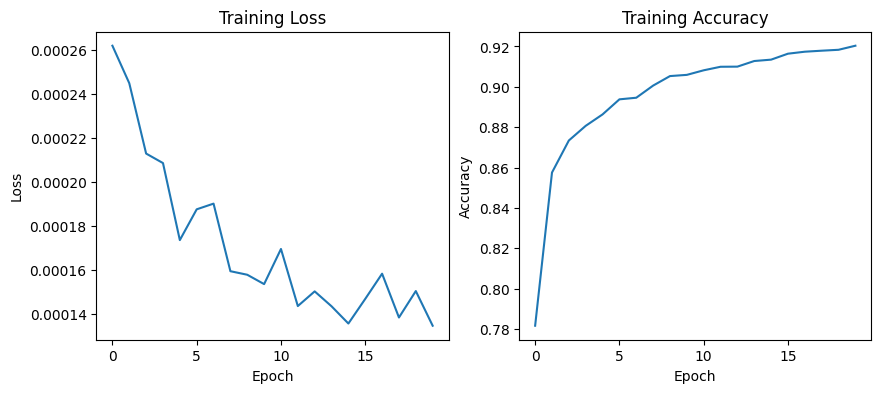
\includegraphics[width=0.8\linewidth]{images/lab2_5_loss.png}
\captionof{figure}{AlexNet Training Losses and Precision Values} % 使用\captionof命令添加标题

\justifying


The model test is visualized below:

\centering % 如果需要居中对齐图像
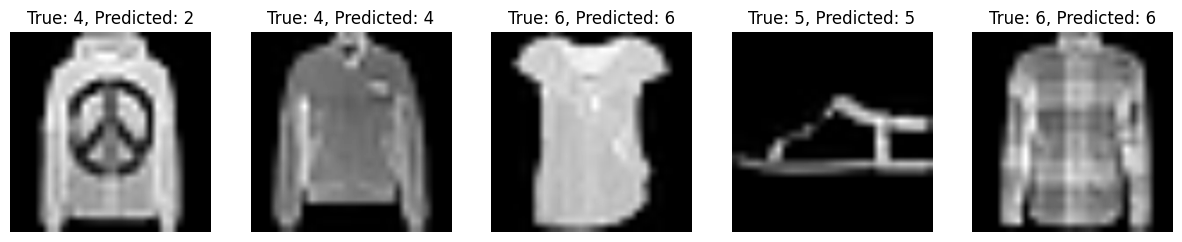
\includegraphics[width=0.8\linewidth]{images/lab2_5_result.png}
\captionof{figure}{AlexNet model test results} % 使用\captionof命令添加标题

\justifying
\subsection{Experimental Summary}
The purpose of this experiment is to evaluate the performance of the AlexNet model on the test set by training it on the FashionMNIST dataset. During the experiment, the data was first preprocessed, including resizing, converting to grayscale images and normalization operations, and the training set data was loaded using the DataLoader. Next, the AlexNetFashionMNIST model was defined and loaded onto the GPU for training. The cross-entropy loss function and Adam optimizer were used for model training, and the average loss and accuracy on the training set were calculated and printed at the end of each epoch. Subsequently, the curves of loss function and accuracy with epoch during the training process were plotted. Finally, the trained model was tested and some randomly selected samples were predicted and visualized. The experimental results show that after 20 epochs of training, AlexNet achieves better performance on the FashionMNIST dataset. The loss function on the training set gradually decreases and the accuracy gradually increases, which verifies that the model gradually converges and learns the features of the data during the training process. Finally, a high accuracy rate is obtained on the test set, which proves the generalization ability and effectiveness of the model. By visualizing the prediction results, the model's prediction of the samples can be observed intuitively, which further validates the performance of the model. In summary, the experimental results show that AlexNet achieves good training and testing performance on the FashionMNIST dataset, proving its effectiveness and applicability in image classification tasks.

\newpage
% 在小结前重新定义格式
\ctexset{
    section={   
        name={Summary},
        format=\bfseries\centering\zihao{-2} % 恢复默认格式
    }
}

\addcontentsline{toc}{section}{Summary}
\section*{Summary}
In this series of experiments, I gradually gained a deeper understanding of the principles and applications of machine learning and deep learning models. I started from the most basic linear regression model, and gradually expanded to linear classification models with network structure, multilayer perceptual machine models, and eventually involved the implementation and application of convolutional neural networks. These experiments not only improved my engineering code skills, but also developed my intuition for tuning parameters.

Initially, I started with experiments on linear regression modeling. Predicting output variables by fitting a linear function is one of the most fundamental models in machine learning. In my experiments, I learned to choose the right loss function and to minimize the loss function using the gradient descent algorithm. These experiments gave me a deeper understanding of the principles and training process of linear regression.

Next, I introduced a linear classification model with a network structure. Compared to simple linear regression models, this model can better cope with complex classification problems. I learned to construct neural networks containing multiple linear layers and activation functions, and to use the cross-entropy loss function for the training of classification tasks. These experiments expanded my knowledge and allowed me to be more flexible in solving various deep learning problems.

I then delved into multilayer perceptual machine modeling. Through the experiments, I gained a deeper understanding of the structure and training methods of MLPs. I learned to choose appropriate activation functions and optimization algorithms, and understood ways to deal with overfitting problems. These experiments not only improved my engineering ability, but also made me more familiar with practical problem solving methods.

Finally, I entered the realm of convolutional neural networks (CNNs). I first learned the basics of convolution, including how convolution operations work and what they do. Then, I explored how to build and train CNN models to solve image classification problems. Through experimentation, I gained insight into the structure of CNNs and the role of convolutional and pooling layers in image processing. I also learned how to use convolutional kernels for feature extraction and build complex classification models with multiple convolutional and fully connected layers.

\addcontentsline{toc}{section}{Acknowledgments}
\section*{Acknowledgments}
I would like to express my special thanks to Mr. Liang for his meticulous guidance and support. Throughout the entire experiment, he not only imparted knowledge of deep learning models and algorithms to me but also patiently answered my questions, which has been incredibly beneficial. Additionally, I would like to thank all the teaching assistants for their hard work and patient guidance during the lab sessions. Their efforts and support have helped me gain a deeper understanding of the course content and provided timely assistance when I encountered difficulties. I am truly grateful for their dedication and support, which have been crucial for my progress. Their contributions will always be remembered and appreciated.

\end{document}